% THIS DOCUMENT IS TAILORED TO REQUIREMENTS FOR SCIENTIFIC COMPUTING.  IT SHOULDN'T
% BE USED FOR NON-SCIENTIFIC COMPUTING PROJECTS
\documentclass[12pt]{article}

\usepackage{amsmath, mathtools}
\usepackage{amsfonts}
\usepackage{amssymb}
\usepackage{graphicx}
\usepackage{colortbl}
\usepackage{xr}
\usepackage{hyperref}
\usepackage{longtable}
\usepackage{xfrac}
\usepackage{tabularx}
\usepackage{float}
\usepackage{siunitx}
\usepackage{booktabs}
\usepackage{caption}
\usepackage{pdflscape}
\usepackage{afterpage}
\usepackage[table,xcdraw]{xcolor}
\usepackage{geometry}
\usepackage{array}
\usepackage{booktabs}
\usepackage{longtable}
\usepackage{enumitem}

\usepackage[round]{natbib}

%\usepackage{refcheck}

\hypersetup{
    bookmarks=true,         % show bookmarks bar?
      colorlinks=true,       % false: boxed links; true: colored links
    linkcolor=red,          % color of internal links (change box color with linkbordercolor)
    citecolor=green,        % color of links to bibliography
    filecolor=magenta,      % color of file links
    urlcolor=cyan           % color of external links
}

%% Comments

\usepackage{color}

\newif\ifcomments\commentstrue %displays comments
%\newif\ifcomments\commentsfalse %so that comments do not display

\ifcomments
\newcommand{\authornote}[3]{\textcolor{#1}{[#3 ---#2]}}
\newcommand{\todo}[1]{\textcolor{red}{[TODO: #1]}}
\else
\newcommand{\authornote}[3]{}
\newcommand{\todo}[1]{}
\fi

\newcommand{\wss}[1]{\authornote{blue}{SS}{#1}} 
\newcommand{\plt}[1]{\authornote{magenta}{TPLT}{#1}} %For explanation of the template
\newcommand{\an}[1]{\authornote{cyan}{Author}{#1}}

%% Common Parts

\newcommand{\progname}{ProgName} % PUT YOUR PROGRAM NAME HERE
\newcommand{\authname}{Team \#, Team Name
\\ Student 1 name
\\ Student 2 name
\\ Student 3 name
\\ Student 4 name} % AUTHOR NAMES                  

\usepackage{hyperref}
    \hypersetup{colorlinks=true, linkcolor=blue, citecolor=blue, filecolor=blue,
                urlcolor=blue, unicode=false}
    \urlstyle{same}
                                

The purpose of reflection questions is to give you a chance to assess your own
learning and that of your group as a whole, and to find ways to improve in the
future. Reflection is an important part of the learning process.  Reflection is
also an essential component of a successful software development process.  

Reflections are most interesting and useful when they're honest, even if the
stories they tell are imperfect. You will be marked based on your depth of
thought and analysis, and not based on the content of the reflections
themselves. Thus, for full marks we encourage you to answer openly and honestly
and to avoid simply writing ``what you think the evaluator wants to hear.''

Please answer the following questions.  Some questions can be answered on the
team level, but where appropriate, each team member should write their own
response:


% For easy change of table widths
\newcommand{\colZwidth}{1.0\textwidth}
\newcommand{\colAwidth}{0.13\textwidth}
\newcommand{\colBwidth}{0.82\textwidth}
\newcommand{\colCwidth}{0.1\textwidth}
\newcommand{\colDwidth}{0.05\textwidth}
\newcommand{\colEwidth}{0.8\textwidth}
\newcommand{\colFwidth}{0.17\textwidth}
\newcommand{\colGwidth}{0.5\textwidth}
\newcommand{\colHwidth}{0.28\textwidth}

% Used so that cross-references have a meaningful prefix
\newcounter{defnum} %Definition Number
\newcommand{\dthedefnum}{GD\thedefnum}
\newcommand{\dref}[1]{GD\ref{#1}}
\newcounter{datadefnum} %Datadefinition Number
\newcommand{\ddthedatadefnum}{DD\thedatadefnum}
\newcommand{\ddref}[1]{DD\ref{#1}}
\newcounter{theorynum} %Theory Number
\newcommand{\tthetheorynum}{TM\thetheorynum}
\newcommand{\tref}[1]{TM\ref{#1}}
\newcounter{tablenum} %Table Number
\newcommand{\tbthetablenum}{TB\thetablenum}
\newcommand{\tbref}[1]{TB\ref{#1}}
\newcounter{assumpnum} %Assumption Number
\newcommand{\atheassumpnum}{A\theassumpnum}
\newcommand{\aref}[1]{A\ref{#1}}
\newcounter{goalnum} %Goal Number
\newcommand{\gthegoalnum}{GS\thegoalnum}
\newcommand{\gsref}[1]{GS\ref{#1}}
\newcounter{instnum} %Instance Number
\newcommand{\itheinstnum}{IM\theinstnum}
\newcommand{\iref}[1]{IM\ref{#1}}
\newcounter{reqnum} %Requirement Number
\newcommand{\rthereqnum}{R\thereqnum}
\newcommand{\rref}[1]{R\ref{#1}}
\newcounter{nfrnum} %NFR Number
\newcommand{\rthenfrnum}{NFR\thenfrnum}
\newcommand{\nfrref}[1]{NFR\ref{#1}}
\newcounter{lcnum} %Likely change number
\newcommand{\lthelcnum}{LC\thelcnum}
\newcommand{\lcref}[1]{LC\ref{#1}}

\usepackage{fullpage}

\newcommand{\deftheory}[9][Not Applicable]
{
\newpage
\noindent \rule{\textwidth}{0.5mm}

\paragraph{RefName: } \textbf{#2} \phantomsection 
\label{#2}

\paragraph{Label:} #3

\noindent \rule{\textwidth}{0.5mm}

\paragraph{Equation:}

#4

\paragraph{Description:}

#5

\paragraph{Notes:}

#6

\paragraph{Source:}

#7

\paragraph{Ref.\ By:}

#8

\paragraph{Preconditions for \hyperref[#2]{#2}:}
\label{#2_precond}

#9

\paragraph{Derivation for \hyperref[#2]{#2}:}
\label{#2_deriv}

#1

\noindent \rule{\textwidth}{0.5mm}

}

\begin{document}

\title{Software Requirements Specification for \progname: subtitle describing software} 
\author{\authname}
\date{\today}
	
\maketitle

~\newpage

\pagenumbering{roman}

\tableofcontents

~\newpage

\section*{Revision History}

\begin{tabularx}{\textwidth}{p{3cm}p{2cm}X}
\toprule {\bf Date} & {\bf Version} & {\bf Notes}\\
\midrule
Date 1 & 1.0 & Notes\\
Date 2 & 1.1 & Notes\\
\bottomrule
\end{tabularx}

~\\
\plt{This template is intended for use by CAS 741.  For CAS 741 the template
should be used exactly as given, except the Reflection Appendix can be deleted.
For the capstone course it is a source of ideas, but shouldn't be followed
exactly.  The exception is the reflection appendix.  All capstone SRS documents
should have a refelection appendix.}

~\newpage

\section{Reference Material}

This section records information for easy reference.

\subsection{Table of Units}

Throughout this document SI (Syst\`{e}me International d'Unit\'{e}s) is employed
as the unit system.  In addition to the basic units, several derived units are
used as described below.  For each unit, the symbol is given followed by a
description of the unit and the SI name.
~\newline

\renewcommand{\arraystretch}{1.2}
%\begin{table}[ht]
  \noindent \begin{tabular}{l l l} 
    \toprule		
    \textbf{symbol} & \textbf{unit} & \textbf{SI}\\
    \midrule 
    \si{\metre} & length & metre\\
    \si{\kilogram} & mass	& kilogram\\
    \si{\second} & time & second\\
    \si{\celsius} & temperature & centigrade\\
    \si{\joule} & energy & joule\\
    \si{\watt} & power & watt (W = \si{\joule\per\second})\\
    \bottomrule
  \end{tabular}
  %	\caption{Provide a caption}
%\end{table}

\plt{Only include the units that your SRS actually uses.}

\plt{Derived units, like newtons, pascal, etc, should show their derivation
    (the units they are derived from) if their constituent units are in the
    table of units (that is, if the units they are derived from are used in the
    document).  For instance, the derivation of pascals as
    $\si{\pascal}=\si{\newton\per\square\meter}$ is shown if newtons and m are
    both in the table.  The derivations of newtons would not be shown if kg and
    s are not both in the table.}

\plt{The symbol for units named after people use capital letters, but the name
  of the unit itself uses lower case.  For instance, pascals use the symbol Pa,
  watts use the symbol W, teslas use the symbol T, newtons use the symbol N,
  etc.  The one exception to this is degree Celsius.  Details on writing metric
  units can be found on the 
  \href{https://www.nist.gov/pml/weights-and-measures/writing-metric-units}
  {NIST} web-page.}

\subsection{Table of Symbols}

The table that follows summarizes the symbols used in this document along with
their units.  The choice of symbols was made to be consistent with the heat
transfer literature and with existing documentation for solar water heating
systems.  The symbols are listed in alphabetical order.

\renewcommand{\arraystretch}{1.2}
%\noindent \begin{tabularx}{1.0\textwidth}{l l X}
\noindent \begin{longtable*}{l l p{12cm}} \toprule
\textbf{symbol} & \textbf{unit} & \textbf{description}\\
\midrule 
$A_C$ & \si[per-mode=symbol] {\square\metre} & coil surface area
\\
$A_\text{in}$ & \si[per-mode=symbol] {\square\metre} & surface area over 
which heat is transferred in
\\ 
\bottomrule
\end{longtable*}
\plt{Use your problems actual symbols.  The si package is a good idea to use for
  units.}

\subsection{Abbreviations and Acronyms}

\renewcommand{\arraystretch}{1.2}
\begin{tabular}{l l} 
  \toprule		
  \textbf{symbol} & \textbf{description}\\
  \midrule 
  A & Assumption\\
  DD & Data Definition\\
  GD & General Definition\\
  GS & Goal Statement\\
  IM & Instance Model\\
  LC & Likely Change\\
  PS & Physical System Description\\
  R & Requirement\\
  SRS & Software Requirements Specification\\
  \progname{} & \plt{put an expanded version of your program name here (as appropriate)}\\
  TM & Theoretical Model\\
  \bottomrule
\end{tabular}\\

\plt{Add any other abbreviations or acronyms that you add}

\subsection{Mathematical Notation}

\plt{This section is optional, but should be included for projects that make use
  of notation to convey mathematical information.  For instance, if typographic
  conventions (like bold face font) are used to distinguish matrices, this
  should be stated here.  If symbols are used to show mathematical operations,
  these should be summarized here.  In some cases the easiest way to summarize
  the notation is to point to a text or other source that explains the
  notation.}

\plt{This section was added to the template because some students use very
  domain specific notation.  This notation will not be readily understandable to
  people outside of your domain.  It should be explained.}

\newpage

\pagenumbering{arabic}

\plt{This SRS template is based on \citet{SmithAndLai2005, SmithEtAl2007,
  SmithAndKoothoor2016}.  It will get you started.  You should not modify the
  section headings, without first discussing the change with the course
  instructor.  Modification means you are not following the template, which
  loses some of the advantage of a template, especially standardization.
  Although the bits shown below do not include type information, you may need to
  add this information for your problem.  If you are unsure, please can ask the
  instructor.}

\plt{Feel free to change the appearance of the report by modifying the LaTeX
  commands.}

\plt{This template document assumes that a single program is being documented.
  If you are documenting a family of models, you should start with a commonality
  analysis.  A separate template is provided for this.  For program
  families you should look at \cite{Smith2006, SmithMcCutchanAndCarette2017}.
  Single family member programs are often programs based on a single physical
  model.  General purpose tools are usually documented as a family.  Families of
  physical models also come up.}

\plt{The SRS is not generally written, or read, sequentially.  The SRS is a
  reference document.  It is generally read in an ad hoc order, as the need
  arises.  For writing an SRS, and for reading one for the first time, the
  suggested order of sections is:
\begin{itemize}
\item Goal Statement
\item Instance Models
\item Requirements
\item Introduction
\item Specific System Description
\end{itemize}
}

\plt{Guiding principles for the SRS document:
\begin{itemize}
\item Do not repeat the same information at the same abstraction level.  If
  information is repeated, the repetition should be at a different abstraction
  level.  For instance, there will be overlap between the scope section and the
  assumptions, but the scope section will not go into as much detail as the
  assumptions section.
\end{itemize}
}

\plt{The template description comments should be disabled before submitting this
  document for grading.}

\plt{You can borrow any wording from the text given in the template.  It is part
  of the template, and not considered an instance of academic integrity.  Of
  course, you need to cite the source of the template.}

\plt{When the documentation is done, it should be possible to trace back to the
  source of every piece of information.  Some information will come from
  external sources, like terminology.  Other information will be derived, like
  General Definitions.}

\plt{An SRS document should have the following qualities: unambiguous,
  consistent, complete, validatable, abstract and traceable.}

\plt{The overall goal of the SRS is that someone that meets the Characteristics
  of the Intended Reader (Section~\ref{sec_IntendedReader}) can learn,
  understand and verify the captured domain knowledge.  They should not have to
  trust the authors of the SRS on any statements.  They should be able to
  independently verify/derive every statement made.}

\section{Introduction}

\plt{The introduction section is written to introduce the problem.  It starts
  general and focuses on the problem domain. The general advice is to start with
a paragraph or two that describes the problem, followed by a ``roadmap''
paragraph.  A roadmap orients the reader by telling them what sub-sections to
expect in the Introduction section.}

\subsection{Purpose of Document}

\plt{This section summarizes the purpose of the SRS document.  It does not focus
  on the problem itself.  The problem is described in the ``Problem
  Description'' section (Section~\ref{Sec_pd}).  The purpose is for the document
  in the context of the project itself, not in the context of this course.
  Although the ``purpose'' of the document is to get a grade, you should not
  mention this.  Instead, ``fake it'' as if this is a real project.  The purpose
  section will be similar between projects.  The purpose of the document is the
  purpose of the SRS, including communication, planning for the design stage,
  etc.}

\subsection{Scope of Requirements} 

\plt{Modelling the real world requires simplification.  The full complexity of
  the actual physics, chemistry, biology is too much for existing models, and
  for existing computational solution techniques.  Rather than say what is in
  the scope, it is usually easier to say what is not.  You can think of it as
  the scope is initially everything, and then it is constrained to create the
  actual scope.  For instance, the problem can be restricted to 2 dimensions, or
  it can ignore the effect of temperature (or pressure) on the material
  properties, etc.}  

\plt{The scope section is related to the assumptions section
  (Section~\ref{sec_assumpt}).  However, the scope and the assumptions are not
  at the same level of abstraction.  The scope is at a high level.  The focus is
  on the ``big picture'' assumptions.  The assumptions section lists, and
  describes, all of the assumptions.}

\plt{The scope section is relevant for later determining typical values of inputs. The scope should make it clear what inputs are reasonable to expect. This is a distinction between scope and context (context is a later section).  Scope affects the inputs while context affects how the software will be used.}

\subsection{Characteristics of Intended Reader} \label{sec_IntendedReader}

\plt{This section summarizes the skills and knowledge of the readers of the
  SRS.  It does NOT have the same purpose as the ``User Characteristics''
  section (Section~\ref{SecUserCharacteristics}).  The intended readers are the
  people that will read, review and maintain the SRS.  They are the people that
  will conceivably design the software that is intended to meet the
  requirements.  The user, on the other hand, is the person that uses the
  software that is built.  They may never read this SRS document.  Of course,
  the same person could be a ``user'' and an ``intended reader.''}

\plt{The intended reader characteristics should be written as unambiguously and
  as specifically as possible.  Rather than say, the user should have an
  understanding of physics, say what kind of physics and at what level.  For
  instance, is high school physics adequate, or should the reader have had a
  graduate course on advanced quantum mechanics?}

\subsection{Organization of Document}

\plt{This section provides a roadmap of the SRS document.  It will help the
  reader orient themselves.  It will provide direction that will help them
  select which sections they want to read, and in what order.  This section will
  be similar between project.}

\section{General System Description}

This section provides general information about the system.  It identifies the
interfaces between the system and its environment, describes the user
characteristics and lists the system constraints.  \plt{This text can likely be
  borrowed verbatim.}

\plt{The purpose of this section is to provide general information about the
  system so the specific requirements in the next section will be easier to
  understand. The general system description section is designed to be
  changeable independent of changes to the functional requirements documented in
  the specific system description. The general system description provides a
  context for a family of related models.  The general description can stay the
  same, while specific details are changed between family members.}

\subsection{System Context}

\plt{Your system context will include a figure that shows the abstract view of
  the software.  Often in a scientific context, the program can be viewed
  abstractly following the design pattern of Inputs $\rightarrow$ Calculations
  $\rightarrow$ Outputs.  The system context will therefore often follow this
  pattern.  The user provides inputs, the system does the calculations, and then
  provides the outputs to the user.  The figure should not show all of the
  inputs, just an abstract view of the main categories of inputs (like material
  properties, geometry, etc.).  Likewise, the outputs should be presented from
  an abstract point of view.  In some cases the diagram will show other external
  entities, besides the user.  For instance, when the software product is a
  library, the user will be another software program, not an actual end user.
  If there are system constraints that the software must work with external
  libraries, these libraries can also be shown on the System Context diagram.
  They should only be named with a specific library name if this is required by
  the system constraint.}

\begin{figure}[h!]
\begin{center}
 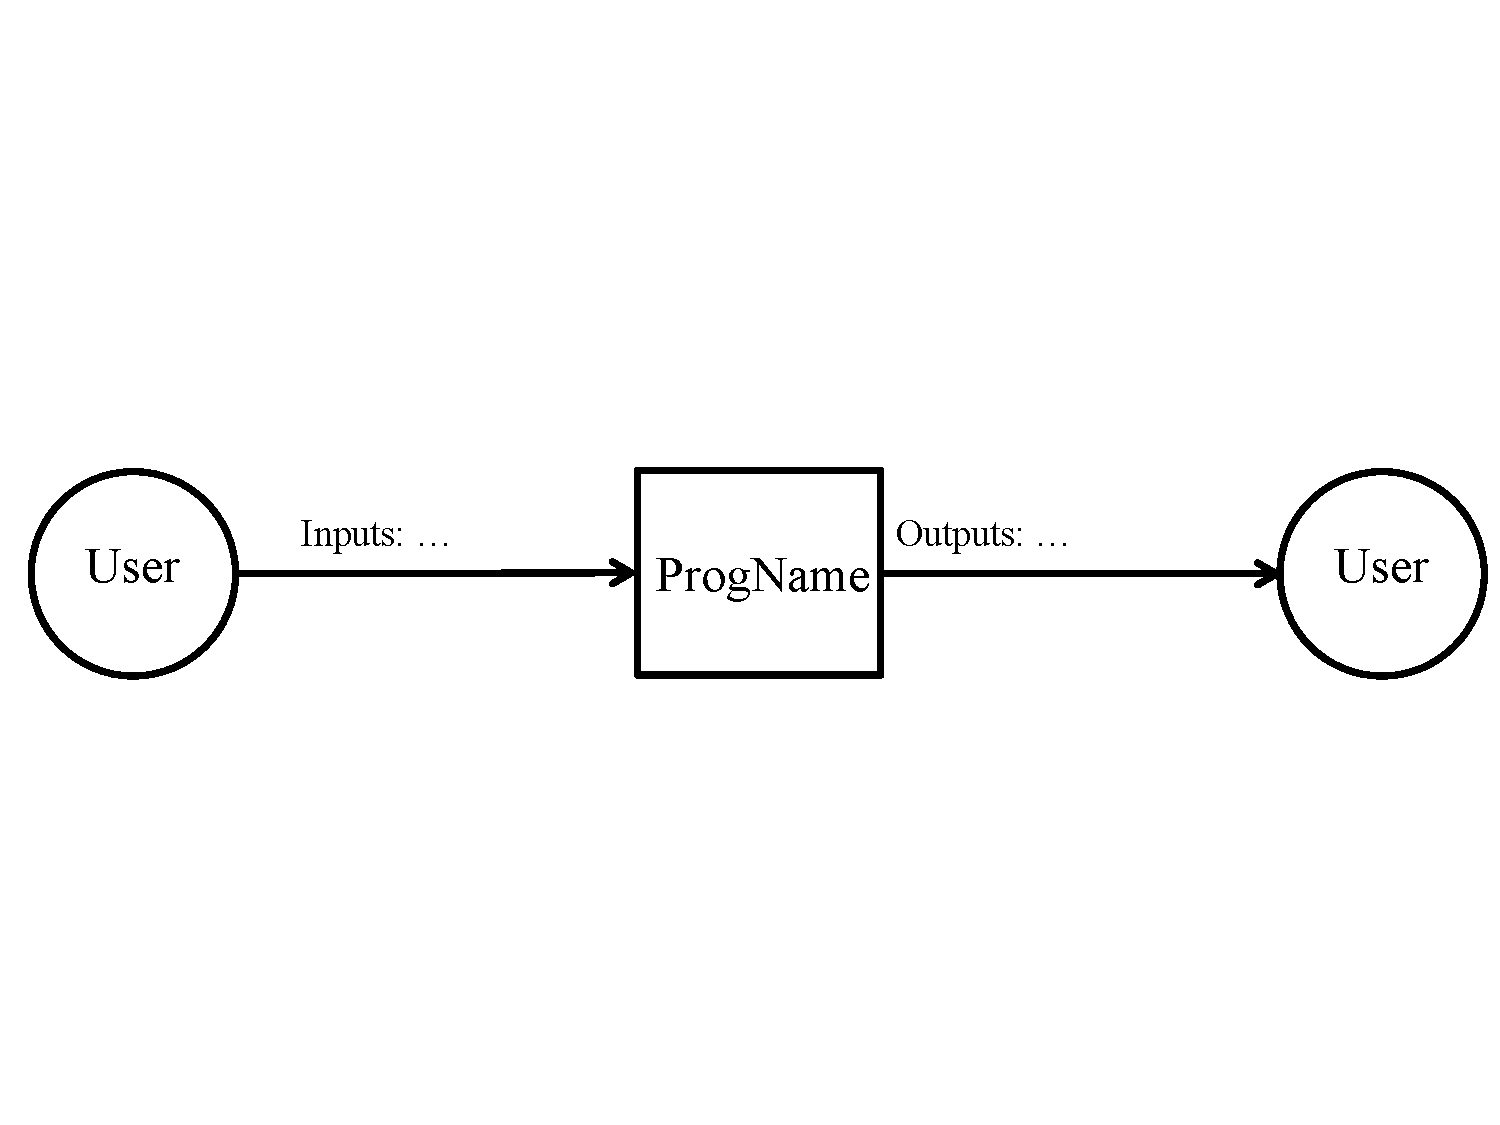
\includegraphics[width=0.6\textwidth]{SystemContextFigure}
\caption{System Context}
\label{Fig_SystemContext} 
\end{center}
\end{figure}

\plt{For each of the entities in the system context diagram its responsibilities
  should be listed.  Whenever possible the system should check for data quality,
  but for some cases the user will need to assume that responsibility.  The list
  of responsibilities should be about the inputs and outputs only, and they
  should be abstract.  Details should not be presented here.  However, the
  information should not be so abstract as to just say ``inputs'' and
  ``outputs''.  A summarizing phrase can be used to characterize the inputs.
  For instance, saying ``material properties'' provides some information, but it
  stays away from the detail of listing every required properties.}

\begin{itemize}
\item User Responsibilities:
\begin{itemize}
\item 
\end{itemize}
\item \progname{} Responsibilities:
\begin{itemize}
\item Detect data type mismatch, such as a string of characters instead of a
  floating point number
\item 
\end{itemize}
\end{itemize}

\plt{Identify in what context the software will typically be used.  Is it for
exploration? education? engineering work? scientific work?. Identify whether it
will be used for mission-critical or safety-critical applications.} \plt{This
additional context information is needed to determine how much effort should be
devoted to the rationale section.  If the application is safety-critical, the
bar is higher.  This is currently less structured, but analogous to, the idea to
the Automotive Safety Integrity Levels (ASILs) that McSCert uses in their
automotive hazard analyses.}

\wss{The }
\subsection{User Characteristics} \label{SecUserCharacteristics}

\plt{This section summarizes the knowledge/skills expected of the user.
  Measuring usability, which is often a required non-function requirement,
  requires knowledge of a typical user.  As mentioned above, the user is a
  different role from the ``intended reader,'' as given in
  Section~\ref{sec_IntendedReader}.  As in Section~\ref{sec_IntendedReader}, the
  user characteristics should be specific an unambiguous.  For instance, ``The
  end user of \progname{} should have an understanding of undergraduate Level 1
  Calculus and Physics.''}

\subsection{System Constraints}

\plt{System constraints differ from other type of requirements because they
  limit the developers' options in the system design and they identify how the
  eventual system must fit into the world. This is the only place in the SRS
  where design decisions can be specified.  That is, the quality requirement for
  abstraction is relaxed here.  However, system constraints should only be
  included if they are truly required.}

\section{Specific System Description}

This section first presents the problem description, which gives a high-level
view of the problem to be solved.  This is followed by the solution characteristics
specification, which presents the assumptions, theories, definitions and finally
the instance models.  \plt{Add any project specific details that are relevant
  for the section overview.}

\subsection{Problem Description} \label{Sec_pd}

\progname{} is intended to solve ... \plt{What problem does your program solve?
The description here should be in the problem space, not the solution space.}

\subsubsection{Terminology and  Definitions}

\plt{This section is expressed in words, not with equations.  It provide the
  meaning of the different words and phrases used in the domain of the problem.
The terminology is used to introduce concepts from the world outside of the
mathematical model  The terminology provides a real world connection to give the
mathematical model meaning.}

This subsection provides a list of terms that are used in the subsequent
sections and their meaning, with the purpose of reducing ambiguity and making it
easier to correctly understand the requirements:

\begin{itemize}

\item 

\end{itemize}

\subsubsection{Physical System Description} \label{sec_phySystDescrip}

\plt{The purpose of this section is to clearly and unambiguously state the
  physical system that is to be modelled. Effective problem solving requires a
  logical and organized approach. The statements on the physical system to be
  studied should cover enough information to solve the problem. The physical
  description involves element identification, where elements are defined as
  independent and separable items of the physical system. Some example elements
  include acceleration due to gravity, the mass of an object, and the size and
  shape of an object. Each element should be identified and labelled, with their
  interesting properties specified clearly. The physical description can also
  include interactions of the elements, such as the following: i) the
  interactions between the elements and their physical environment; ii) the
  interactions between elements; and, iii) the initial or boundary conditions.}

\plt{The elements of the physical system do not have to correspond to an actual
physical entity.  They can be conceptual.  This is particularly important when
the documentation is for a numerical method. }

The physical system of \progname{}, as shown in Figure~?,
includes the following elements:

\begin{itemize}

\item[PS1:] 

\item[PS2:] ...

\end{itemize}

\plt{A figure here makes sense for most SRS documents}

% \begin{figure}[h!]
% \begin{center}
% %\rotatebox{-90}
% {
%  \includegraphics[width=0.5\textwidth]{<FigureName>}
% }
% \caption{\label{<Label>} <Caption>}
% \end{center}
% \end{figure}

\subsubsection{Goal Statements}

\plt{The goal statements refine the ``Problem Description''
  (Section~\ref{Sec_pd}).  A goal is a functional objective the system under
  consideration should achieve. Goals provide criteria for sufficient
  completeness of a requirements specification and for requirements
  pertinence. Goals will be refined in Section “Instanced Models”
  (Section~\ref{sec_instance}). Large and complex goals should be decomposed
  into smaller sub-goals.  The goals are written abstractly, with a minimal
  amount of technical language.  They should be understandable by non-domain
  experts.}

\noindent Given the \plt{inputs}, the goal statements are:

\begin{itemize}

\item[GS\refstepcounter{goalnum}\thegoalnum \label{G_meaningfulLabel}:] \plt{One
    sentence description of the goal.  There may be more than one.  Each Goal
    should have a meaningful label.}

\end{itemize}

\subsection{Solution Characteristics Specification}

\plt{This section specifies the information in the solution domain of the system
  to be developed. This section is intended to express what is required in
  such a way that analysts and stakeholders get a clear picture, and the
  latter will accept it. The purpose of this section is to reduce the problem
  into one expressed in mathematical terms. Mathematical expertise is used to
  extract the essentials from the underlying physical description of the
  problem, and to collect and substantiate all physical data pertinent to the
  problem.}

\plt{This section presents the solution characteristics by successively refining
  models.  It starts with the abstract/general Theoretical Models (TMs) and
  refines them to the concrete/specific Instance Models (IMs).  If necessary
  there are intermediate refinements to General Definitions (GDs).  All of these
  refinements can potentially use Assumptions (A) and Data Definitions (DD).
  TMs are refined to create new models, that are called GMs or IMs. DDs are not
  refined; they are just used. GDs and IMs are derived, or refined, from other
  models. DDs are not derived; they are just given. TMs are also just given, but
  they are refined, not used.  If a potential DD includes a derivation, then
  that means it is refining other models, which would make it a GD or an IM.}

\plt{The above makes a distinction between ``refined'' and ``used.'' A model is
  refined to another model if it is changed by the refinement. When we change a
  general 3D equation to a 2D equation, we are making a refinement, by applying
  the assumption that the third dimension does not matter. If we use a
  definition, like the definition of density, we aren't refining, or changing
  that definition, we are just using it.}

\plt{The same information can be a TM in one problem and a DD in another.  It is
  about how the information is used.  In one problem the definition of
  acceleration can be a TM, in another it would be a DD.}

\plt{There is repetition between the information given in the different chunks
  (TM, GDs etc) with other information in the document.  For instance, the
  meaning of the symbols, the units etc are repeated.  This is so that the
  chunks can stand on their own when being read by a reviewer/user.  It also
  facilitates reuse of the models in a different context.}

\noindent \plt{The relationships between the parts of the document are show in
  the following figure.  In this diagram ``may ref'' has the same role as
  ``uses'' above.  The figure adds ``Likely Changes,'' which are able to
  reference (use) Assumptions.}

\begin{figure}[H]
  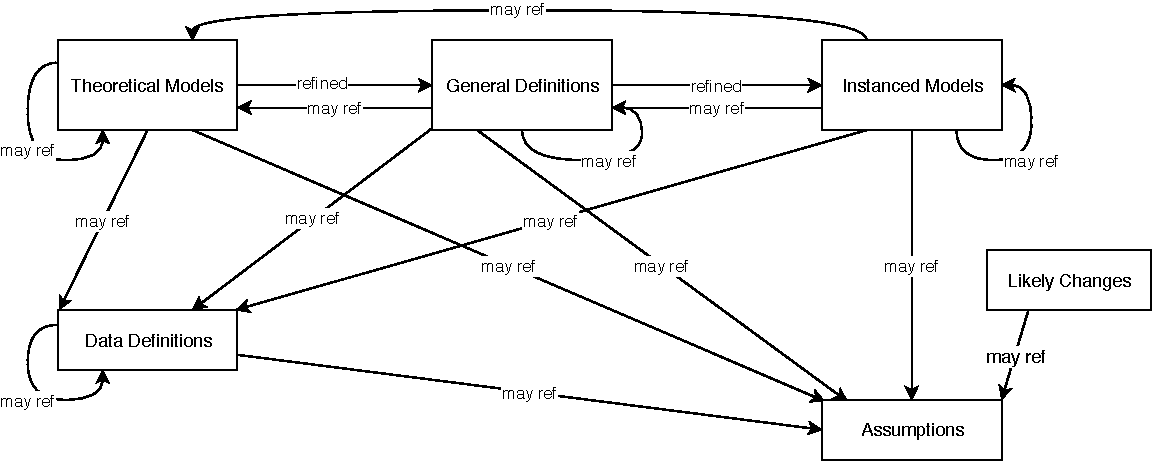
\includegraphics[scale=0.9]{RelationsBetweenTM_GD_IM_DD_A.pdf}
\end{figure}

The instance models that govern \progname{} are presented in
Subsection~\ref{sec_instance}.  The information to understand the meaning of the
instance models and their derivation is also presented, so that the instance
models can be verified.

\subsubsection{Types}

\plt{This section is optional. Defining types can make the document easier to
understand.}

\subsubsection{Scope Decisions}

\plt{This section is optional.}
\subsubsection{Modelling Decisions}

\plt{This section is optional.}

\subsubsection{Assumptions} \label{sec_assumpt}

\plt{The assumptions are a refinement of the scope.  The scope is general, where
  the assumptions are specific.  All assumptions should be listed, even those
  that domain experts know so well that they are rarely (if ever) written down.}
\plt{The document should not take for granted that the reader knows which
  assumptions have been made. In the case of unusual assumptions, it is
  recommended that the documentation either include, or point to, an explanation
  and justification for the assumption.}
\plt{If it helps with the organization and understandability, the assumptions can be presented as sub sections.  The following sub-sections are options: background theory assumptions, helper theory assumptions, generic theory assumptions, problem specific assumptions, and rationale assumptions}

This section simplifies the original problem and helps in developing the
theoretical model by filling in the missing information for the physical system.
The numbers given in the square brackets refer to the theoretical model [TM],
general definition [GD], data definition [DD], instance model [IM], or likely
change [LC], in which the respective assumption is used.

\begin{itemize}

\item[A\refstepcounter{assumpnum}\theassumpnum \label{A_meaningfulLabel}:]
  \plt{Short description of each assumption.  Each assumption
    should have a meaningful label.  Use cross-references to identify the
    appropriate traceability to TM, GD, DD etc., using commands like dref, ddref
    etc.  Each assumption should be atomic - that is, there should not be an
    explicit (or implicit) ``and'' in the text of an assumption.}

\end{itemize}

\subsubsection{Theoretical Models}\label{sec_theoretical}

\plt{Theoretical models are sets of abstract mathematical equations or axioms
  for solving the problem described in Section ``Physical System Description''
  (Section~\ref{sec_phySystDescrip}). Examples of theoretical models are
  physical laws, constitutive equations, relevant conversion factors, etc.}

\plt{Optionally the theory section could be divided into subsections to provide more structure and improve understandability and reusability.  Potential subsections include the following: Context theories, background theories, helper theories, generic theories, problem specific theories, final theories and rationale theories.}

This section focuses on the general equations and laws that \progname{} is based
on.  \plt{Modify the examples below for your problem, and add additional models
  as appropriate.}

~\newline

\noindent
\deftheory
% #2 refname of theory
{TM:COE}
% #3 label
{Conservation of thermal energy}
% #4 equation
{
  $-{\bf \nabla \cdot q} + g$ = $\rho C \frac{\partial T}{\partial t}$
}
% #5 description
{
  The above equation gives the conservation of energy for transient heat transfer in a material
  of specific heat capacity $C$ (\si{\joule\per\kilogram\per\celsius}) and density $\rho$ 
  (\si{\kilogram\per\cubic\metre}), where $\bf q$ is the thermal flux vector (\si{\watt\per\square\metre}),
  $g$ is the volumetric heat generation
  (\si{\watt\per\cubic\metre}), $T$ is the temperature
  (\si{\celsius}),  $t$ is time (\si{\second}), and $\nabla$ is
  the gradient operator.  For this equation to apply, other forms
  of energy, such as mechanical energy, are assumed to be negligible in the
  system (\aref{A_OnlyThermalEnergy}).  In general, the material properties ($\rho$ and $C$) depend on temperature.
}
% #6 Notes
{
None.
}
% #7 Source
{
  \url{http://www.efunda.com/formulae/heat_transfer/conduction/overview_cond.cfm}
}
% #8 Referenced by
{
  \dref{ROCT}
}
% #9 Preconditions
{
None
}
% #1 derivation - not applicable by default
{}

\plt{``Ref.\ By'' is used repeatedly with the different types of information.
  This stands for Referenced By.  It means that the models, definitions and
  assumptions listed reference the current model, definition or assumption.
  This information is given for traceability.  Ref. By provides a pointer in the
  opposite direction to what we commonly do.  You still need to have a reference
  in the other direction pointing to the current model, definition or
  assumption.  As an example, if TM1 is referenced by GD2, that means that GD2 will
  explicitly include a reference to TM1.}

~\newline

\subsubsection{General Definitions}\label{sec_gendef}

\plt{General Definitions (GDs) are a refinement of one or more TMs, and/or of
  other GDs.  The GDs are less abstract than the TMs.  Generally the reduction
  in abstraction is possible through invoking (using/referencing) Assumptions.
  For instance, the TM could be Newton's Law of Cooling stated abstracting.  The
  GD could take the general law and apply it to get a 1D equation.}

This section collects the laws and equations that will be used in building the
instance models.

\plt{Some projects may not have any content for this section, but the section
  heading should be kept.}  \plt{Modify the examples below for your problem, and
  add additional definitions as appropriate.}

~\newline

\noindent
\begin{minipage}{\textwidth}
\renewcommand*{\arraystretch}{1.5}
\begin{tabular}{| p{\colAwidth} | p{\colBwidth}|}
\hline
\rowcolor[gray]{0.9}
Number& GD\refstepcounter{defnum}\thedefnum \label{NL}\\
\hline
Label &\bf Newton's law of cooling \\
\hline
% Units&$MLt^{-3}T^0$\\
% \hline
SI Units&\si{\watt\per\square\metre}\\
\hline
Equation&$ q(t) = h \Delta T(t)$  \\
\hline
Description &
Newton's law of cooling describes convective cooling from a surface.  The law is
stated as: the rate of heat loss from a body is proportional to the difference
in temperatures between the body and its surroundings.
\\
& $q(t)$ is the thermal flux (\si{\watt\per\square\metre}).\\
& $h$ is the heat transfer coefficient, assumed independent of $T$ (\aref{A_hcoeff})
	(\si{\watt\per\square\metre\per\celsius}).\\
&$\Delta T(t)$= $T(t) - T_{\text{env}}(t)$ is the time-dependent thermal gradient
between the environment and the object (\si{\celsius}).
\\
\hline
  Source & Citation here \\
  \hline
  Ref.\ By & \ddref{FluxCoil}, \ddref{FluxPCM}\\
  \hline
\end{tabular}
\end{minipage}\\

\subsubsection*{Detailed derivation of simplified rate of change of temperature}

\plt{This may be necessary when the necessary information does not fit in the
  description field.}
\plt{Derivations are important for justifying a given GD.  You want it to be
  clear where the equation came from.}

\subsubsection{Data Definitions}\label{sec_datadef}

\plt{The Data Definitions are definitions of symbols and equations that are
  given for the problem.  They are not derived; they are simply used by other
  models.  For instance, if a problem depends on density, there may be a data
  definition for the equation defining density.  The DDs are given information
  that you can use in your other modules.}

\plt{All Data Definitions should be used (referenced) by at least one other
  model.}

This section collects and defines all the data needed to build the instance
models. The dimension of each quantity is also given.  \plt{Modify the examples
  below for your problem, and add additional definitions as appropriate.}

~\newline

\noindent
\begin{minipage}{\textwidth}
\renewcommand*{\arraystretch}{1.5}
\begin{tabular}{| p{\colAwidth} | p{\colBwidth}|}
\hline
\rowcolor[gray]{0.9}
Number& DD\refstepcounter{datadefnum}\thedatadefnum \label{FluxCoil}\\
\hline
Label& \bf Heat flux out of coil\\
\hline
Symbol &$q_C$\\
\hline
% Units& $Mt^{-3}$\\
% \hline
  SI Units & \si{\watt\per\square\metre}\\
  \hline
  Equation&$q_C(t) = h_C (T_C - T_W(t))$, over area $A_C$\\
  \hline
  Description & 
                $T_C$ is the temperature of the coil (\si{\celsius}).  $T_W$ is the temperature of the water (\si{\celsius}).  
                The heat flux out of the coil, $q_C$ (\si{\watt\per\square\metre}), is found by
                assuming that Newton's Law 
                of Cooling applies (\aref{A_Newt_coil}).  This law (\dref{NL}) is used on the surface of
                the coil, which has area $A_C$ (\si{\square\metre}) and heat 
                transfer coefficient $h_C$
                (\si{\watt\per\square\metre\per\celsius}).  This equation
                assumes that the temperature of the coil is constant over time (\aref{A_tcoil}) and that it does not vary along the length
                of the coil (\aref{A_tlcoil}).
  \\
  \hline
  Sources& Citation here \\
  \hline
  Ref.\ By & \iref{ewat}\\
  \hline
\end{tabular}
\end{minipage}\\

\subsubsection{Data Types}\label{sec_datatypes}

\plt{This section is optional.  In many scientific computing programs it isn't
  necessary, since the inputs and outpus are straightforward types, like reals,
  integers, and sequences of reals and integers.  However, for some problems it
  is very helpful to capture the type information.}

\plt{The data types are not derived; they are simply stated and used by other
  models.}

\plt{All data types must be used by at least one of the models.}

\plt{For the mathematical notation for expressing types, the recommendation is
  to use the notation of~\citet{HoffmanAndStrooper1995}.}

This section collects and defines all the data types needed to document the
models. \plt{Modify the examples below for your problem, and add additional
  definitions as appropriate.}

~\newline

\noindent
\begin{minipage}{\textwidth}
\renewcommand*{\arraystretch}{1.5}
\begin{tabular}{| p{\colAwidth} | p{\colBwidth}|}
  \hline
  \rowcolor[gray]{0.9}
  Type Name & Name for Type\\
  \hline
  Type Def & mathematical definition of the type\\
  \hline
  Description & description here
  \\
  \hline
  Sources & Citation here, if the type is borrowed from another source\\
  \hline
\end{tabular}
\end{minipage}\\

\subsubsection{Instance Models} \label{sec_instance}    

\plt{The motivation for this section is to reduce the problem defined in
  ``Physical System Description'' (Section~\ref{sec_phySystDescrip}) to one
  expressed in mathematical terms. The IMs are built by refining the TMs and/or
  GDs.  This section should remain abstract.  The SRS should specify the
  requirements without considering the implementation.}

This section transforms the problem defined in Section~\ref{Sec_pd} into 
one which is expressed in mathematical terms. It uses concrete symbols defined 
in Section~\ref{sec_datadef} to replace the abstract symbols in the models 
identified in Sections~\ref{sec_theoretical} and~\ref{sec_gendef}.

The goals \plt{reference your goals} are solved by \plt{reference your instance
  models}.  \plt{other details, with cross-references where appropriate.}
\plt{Modify the examples below for your problem, and add additional models as
  appropriate.}

~\newline

%Instance Model 1

\noindent
\begin{minipage}{\textwidth}
\renewcommand*{\arraystretch}{1.5}
\begin{tabular}{| p{\colAwidth} | p{\colBwidth}|}
  \hline
  \rowcolor[gray]{0.9}
  Number& IM\refstepcounter{instnum}\theinstnum \label{ewat}\\
  \hline
  Label& \bf Energy balance on water to find $T_W$\\
  \hline
  Input&$m_W$, $C_W$, $h_C$, $A_C$, $h_P$, $A_P$, $t_\text{final}$, $T_C$, 
  $T_\text{init}$, $T_P(t)$ from \iref{epcm}\\
  & The input is constrained so that $T_\text{init} \leq T_C$ (\aref{A_charge})\\
  \hline
  Output&$T_W(t)$, $0\leq t \leq t_\text{final}$, such that\\
  &$\frac{dT_W}{dt} = \frac{1}{\tau_W}[(T_C - T_W(t)) + {\eta}(T_P(t) - T_W(t))]$,\\
  &$T_W(0) = T_P(0) = T_\text{init}$ (\aref{A_InitTemp}) and $T_P(t)$ from \iref{epcm} \\
  \hline
  Description&$T_W$ is the water temperature (\si{\celsius}).\\
  &$T_P$ is the PCM temperature (\si{\celsius}).\\
  &$T_C$ is the coil temperature (\si{\celsius}).\\
  &$\tau_W = \frac{m_W C_W}{h_C A_C}$ is a constant (\si{\second}).\\
  &$\eta = \frac{h_P A_P}{h_C A_C}$ is a constant (dimensionless).\\
  & The above equation applies as long as the water is in liquid form,
  $0<T_W<100^o\text{C}$, where $0^o\text{C}$ and $100^o\text{C}$ are the melting
  and boiling points of water, respectively (\aref{A_OpRange}, \aref{A_Pressure}).
  \\
  \hline
  Sources& Citation here \\
  \hline
  Ref.\ By & \iref{epcm}\\
  \hline
\end{tabular}
\end{minipage}\\

%~\newline

\subsubsection*{Derivation of ...}

\plt{The derivation shows how the IM is derived from the TMs/GDs.  In cases
  where the derivation cannot be described under the Description field, it will
  be necessary to include this subsection.}

\subsubsection{Input Data Constraints} \label{sec_DataConstraints}    

Table~\ref{TblInputVar} shows the data constraints on the input output
variables.  The column for physical constraints gives the physical limitations
on the range of values that can be taken by the variable.  The column for
software constraints restricts the range of inputs to reasonable values.  The
software constraints will be helpful in the design stage for picking suitable
algorithms.  The constraints are conservative, to give the user of the model the
flexibility to experiment with unusual situations.  The column of typical values
is intended to provide a feel for a common scenario.  The uncertainty column
provides an estimate of the confidence with which the physical quantities can be
measured.  This information would be part of the input if one were performing an
uncertainty quantification exercise.

The specification parameters in Table~\ref{TblInputVar} are listed in
Table~\ref{TblSpecParams}.

\begin{table}[!h]
  \caption{Input Variables} \label{TblInputVar}
  \renewcommand{\arraystretch}{1.2}
\noindent \begin{longtable*}{l l l l c} 
  \toprule
  \textbf{Var} & \textbf{Physical Constraints} & \textbf{Software Constraints} &
                             \textbf{Typical Value} & \textbf{Uncertainty}\\
  \midrule 
  $L$ & $L > 0$ & $L_{\text{min}} \leq L \leq L_{\text{max}}$ & 1.5 \si[per-mode=symbol] {\metre} & 10\%
  \\
  \bottomrule
\end{longtable*}
\end{table}

\noindent 
\begin{description}
\item[(*)] \plt{you might need to add some notes or clarifications}
\end{description}

\begin{table}[!h]
\caption{Specification Parameter Values} \label{TblSpecParams}
\renewcommand{\arraystretch}{1.2}
\noindent \begin{longtable*}{l l} 
  \toprule
  \textbf{Var} & \textbf{Value} \\
  \midrule 
  $L_\text{min}$ & 0.1 \si{\metre}\\
  \bottomrule
\end{longtable*}
\end{table}

\subsubsection{Properties of a Correct Solution} \label{sec_CorrectSolution}

\noindent
A correct solution must exhibit \plt{fill in the details}.  \plt{These
  properties are in addition to the stated requirements.  There is no need to
  repeat the requirements here.  These additional properties may not exist for
  every problem.  Examples include conservation laws (like conservation of
  energy or mass) and known constraints on outputs, which are usually summarized
  in tabular form.  A sample table is shown in Table~\ref{TblOutputVar}}

\begin{table}[!h]
\caption{Output Variables} \label{TblOutputVar}
\renewcommand{\arraystretch}{1.2}
\noindent \begin{longtable*}{l l} 
  \toprule
  \textbf{Var} & \textbf{Physical Constraints} \\
  \midrule 
  $T_W$ & $T_\text{init} \leq T_W \leq T_C$ (by~\aref{A_charge})
  \\
  \bottomrule
\end{longtable*}
\end{table}

\plt{This section is not for test cases or techniques for verification and
  validation.  Those topics will be addressed in the Verification and Validation
  plan.}

  \clearpage
\section{Functional Requirements}
This section provides the functional requirements, the business tasks that the
software is expected to complete, and the nonfunctional requirements, the
qualities that the software is expected to exhibit.

\begin{table}[h!]
\centering
\rowcolors{2}{white}{white} % All rows except the first will be white
\begin{tabular}{|p{3.5cm}|p{11.5cm}|}
\hline
\rowcolor{gray!30} % Light gray for the first row (header)
\textbf{FR1} & The system shall accept chest X-ray images as input from authorized users, including healthcare professionals and patients. \\
\hline
\textbf{Rationale} & To perform analysis, the system requires chest X-ray images to be uploaded by users in supported formats (DICOM, JPEG, PNG). \\
\hline
\textbf{Verification} & Test the upload functionality with different image formats and ensure the system can process the images without errors. \\
\hline
\textbf{Priority} & High \\
\hline
\textbf{Traceability} & R\refstepcounter{reqnum}\thereqnum \label{R_Inputs} \\
\hline
\end{tabular}
\caption{Functional Requirement FR1}
\centering
\rowcolors{2}{white}{white}
\begin{tabular}{|p{3.5cm}|p{11.5cm}|}
\hline
\rowcolor{gray!30}
\textbf{FR2} & The system shall enable users to input additional patient symptoms, such as cough, chest pain, or fever. \\
\hline
\textbf{Rationale} & Including patient symptoms helps provide more context for the AI model to enhance disease detection accuracy. Our goal is to make the AI more useful by giving it more information to work with. \\
\hline
\textbf{Verification} & Verify that users can enter patient symptoms and that they are correctly linked to the associated X-ray images. \\
\hline
\textbf{Priority} & Medium \\
\hline
\textbf{Traceability} & R\refstepcounter{reqnum}\thereqnum \label{R_Symptoms} \\
\hline
\end{tabular}
\caption{Functional Requirement FR2}
\end{table}
\begin{table}[h!]
\centering
\rowcolors{2}{white}{white}
\begin{tabular}{|p{3.5cm}|p{11.5cm}|}
\hline
\rowcolor{gray!30}
\textbf{FR3} & The system shall analyze chest X-ray images to detect the presence or absence of specific diseases with an accuracy of 85\% or higher. \\
\hline
\textbf{Rationale} & One of the core functionalities of our system is its ability to detect diseases like pneumonia from X-rays. This ensures the AI model is effective in clinical settings. \\
\hline
\textbf{Verification} & Evaluate the accuracy of the disease detection model against a test dataset and confirm it meets or exceeds the 85\% accuracy threshold. \\
\hline
\textbf{Priority} & High \\
\hline
\textbf{Traceability} & R\refstepcounter{reqnum}\thereqnum \label{R_DiseaseDetection} \\
\hline
\end{tabular}
\caption{Functional Requirement FR3}
\end{table}
\begin{table}[h!]
\centering
\rowcolors{2}{white}{white}
\begin{tabular}{|p{3.5cm}|p{11.5cm}|}
\hline
\rowcolor{gray!30}
\textbf{FR4} & The system shall indicate whether a patient's condition has improved, worsened, or remained stable between scans. \\
\hline
\textbf{Rationale} & This feature helps clinicians monitor disease progression or regression, which is vital for evaluating the effectiveness of treatments over time.\\
\hline
\textbf{Verification} & Verify that the system provides a status of the patient's condition after comparing multiple scans. \\
\hline
\textbf{Priority} & High \\
\hline
\textbf{Traceability} & R\refstepcounter{reqnum}\thereqnum \label{R_ConditionStatus} \\
\hline
\end{tabular}
\caption{Functional Requirement FR4}
\end{table}
\begin{table}[h!]
\centering
\rowcolors{2}{white}{white}
\begin{tabular}{|p{3.5cm}|p{11.5cm}|}
\hline
\rowcolor{gray!30}
\textbf{FR5} & The system shall generate visual aids by highlighting affected areas on the chest X-ray images. \\
\hline
\textbf{Rationale} & By highlighting affected regions, our system makes it easier for clinicians to identify the areas of concern in a chest X-ray. This improves their ability to act quickly. \\
\hline
\textbf{Verification} & Ensure that the system overlays the appropriate markers on the X-ray images to highlight abnormal areas. \\
\hline
\textbf{Priority} & Medium\\
\hline
\textbf{Traceability} & R\refstepcounter{reqnum}\thereqnum \label{R_VisualAids} \\
\hline
\end{tabular}
\caption{Functional Requirement FR5}
\end{table}
\begin{table}[h!]
\centering
\rowcolors{2}{white}{white}
\begin{tabular}{|p{3.5cm}|p{11.5cm}|}
\hline
\rowcolor{gray!30}
\textbf{FR6} & The system shall produce a structured, human-readable report summarizing key findings, disease detection results, and progression status. \\
\hline
\textbf{Rationale} & A comprehensive report makes it easier for clinicians to interpret the analysis results, especially in fast-paced environments where time is critical. \\
\hline
\textbf{Verification} & Verify that the system generates a report containing all necessary details in an organized format. \\
\hline
\textbf{Priority} & High \\
\hline
\textbf{Traceability} & R\refstepcounter{reqnum}\thereqnum \label{R_ReportGeneration} \\
\hline
\end{tabular}
\caption{Functional Requirement FR6}
\end{table}
\begin{table}[h!]
\centering
\rowcolors{2}{white}{white}
\begin{tabular}{|p{3.5cm}|p{11.5cm}|}
\hline
\rowcolor{gray!30}
\textbf{FR7} & The system shall store patient data, including images and reports, in a secure database for future reference. \\
\hline
\textbf{Rationale} & Keeping patient records secure and accessible for future consultations or research is important for patient care continuity. \\
\hline
\textbf{Verification} & Verify that the system correctly stores and retrieves patient data from the database. \\
\hline
\textbf{Priority} & Medium \\
\hline
\textbf{Traceability} & R\refstepcounter{reqnum}\thereqnum \label{R_DataStorage} \\
\hline
\end{tabular}
\caption{Functional Requirement FR7}
\end{table}

\begin{table}[h!]
\centering
\rowcolors{2}{white}{white}
\begin{tabular}{|p{3.5cm}|p{11.5cm}|}
\hline
\rowcolor{gray!30}
\textbf{FR8} & The system shall provide alerts to clinicians if significant changes in a patient's condition are detected between scans. \\
\hline
\textbf{Rationale} & Automated alerts can save time and ensure that urgent cases are handled quickly, improving patient outcomes. \\
\hline
\textbf{Verification} & Test that alerts are generated when the system detects a significant change in disease severity or condition. \\
\hline
\textbf{Priority} & Low \\
\hline
\textbf{Traceability} & R\refstepcounter{reqnum}\thereqnum \label{R_Alerts} \\
\hline
\end{tabular}
\caption{Functional Requirement FR8}
\end{table}
\begin{table}[h!]
  \centering
  \rowcolors{2}{white}{white}
  \begin{tabular}{|p{3.5cm}|p{11.5cm}|}
  \hline
  \rowcolor{gray!30}
  \textbf{FR9} & The system shall allow healthcare professionals to adjust treatment plans based on the X-ray analysis results. \\
  \hline
  \textbf{Rationale} & Allowing clinicians to modify treatment plans based on X-ray results helps to tailor patient care more effectively. This ensures that the system supports decision-making in real-time clinical settings. \\
  \hline
  \textbf{Verification} & Verify that healthcare professionals can modify treatment plans directly in the system, and that these changes are linked to the corresponding X-ray analysis results. \\
  \hline
  \textbf{Priority} & High \\
  \hline
  \textbf{Traceability} & R\refstepcounter{reqnum}\thereqnum \label{R_TreatmentAdjustment} \\
  \hline
  \end{tabular}
  \caption{Functional Requirement FR9}
  \end{table}

\begin{table}[h!]
\centering
\rowcolors{2}{white}{white}
\begin{tabular}{|p{3.5cm}|p{11.5cm}|}
\hline
\rowcolor{gray!30}
\textbf{FR10} & The system shall allow integration with electronic health record (EHR) systems to import and export patient data. \\
\hline
\textbf{Rationale} & Integrating with existing EHR systems improves workflow efficiency and reduces the need for manual data entry, making the system more useful in a clinical setting. \\
\hline
\textbf{Verification} & Test the system’s ability to connect with standard EHR systems and exchange data using appropriate protocols. \\
\hline
\textbf{Priority} & Low \\
\hline
\textbf{Traceability} & R\refstepcounter{reqnum}\thereqnum \label{R_EHRIntegration} \\
\hline
\end{tabular}
\caption{Functional Requirement FR10}
\end{table}
\begin{table}[h!]
\centering
\rowcolors{2}{white}{white}
\begin{tabular}{|p{3.5cm}|p{11.5cm}|}
\hline
\rowcolor{gray!30}
\textbf{FR11} & The system shall display confidence levels for disease detection and progression analysis results through an intuitive user interface that requires minimal training to operate. \\
\hline
\textbf{Rationale} & Providing confidence levels helps clinicians assess the reliability of the results. \\
\hline
\textbf{Verification} & Check that the system displays a confidence score alongside each analysis result. \\
\hline
\textbf{Priority} & High \\
\hline
\textbf{Traceability} & R\refstepcounter{reqnum}\thereqnum \label{R_UserInterface} \\
\hline
\end{tabular}
\caption{Functional Requirement FR11}
\end{table}

\begin{table}[h!]
\centering
\rowcolors{2}{white}{white}
\begin{tabular}{|p{3.5cm}|p{11.5cm}|}
\hline
\rowcolor{gray!30}
\textbf{FR12} & The system shall allow patients to upload their own chest X-ray images for self-diagnosis purposes, subject to appropriate disclaimers. \\
\hline
\textbf{Rationale} & Allowing patients to upload their own images increases engagement in their healthcare journey, though it must be made clear that professional interpretation is still necessary. \\
\hline
\textbf{Verification} & Ensure that patients can upload images and that the system displays appropriate disclaimers before analysis. \\
\hline
\textbf{Priority} & Low \\
\hline
\textbf{Traceability} & R\refstepcounter{reqnum}\thereqnum \label{R_PatientUploads} \\
\hline
\end{tabular}
\caption{Functional Requirement FR12}
\end{table}

\begin{table}[h!]
\centering
\rowcolors{2}{white}{white}
\begin{tabular}{|p{3.5cm}|p{11.5cm}|}
\hline
\rowcolor{gray!30}
\textbf{FR13} & The system shall support multiple user roles with appropriate access levels (e.g., physician, radiologist, patient). \\
\hline
\textbf{Rationale} & Different users need access to different features and data, so assigning roles ensures that each user can only perform actions they are authorized to. \\
\hline
\textbf{Verification} & Verify that users are assigned roles and that their access is restricted to the appropriate features based on their role. \\
\hline
\textbf{Priority} & High \\
\hline
\textbf{Traceability} & R\refstepcounter{reqnum}\thereqnum \label{R_UserRoles} \\
\hline
\end{tabular}
\caption{Functional Requirement FR13}
\end{table}
\begin{table}[h!]
\centering
\rowcolors{2}{white}{white}
\begin{tabular}{|p{3.5cm}|p{11.5cm}|}
\hline
\rowcolor{gray!30}
\textbf{FR14} & The system shall create a new copy of a patient’s X-ray before running the AI model for analysis. \\
\hline
\textbf{Rationale} & Creating a new copy ensures that the original X-ray remains unchanged for future reference, while the AI model works on the new version for tagging and analysis. \\
\hline
\textbf{Verification} & Verify that the system creates a new X-ray copy, preserving the original file while the AI model runs on the duplicate. \\
\hline
\textbf{Priority} & High \\
\hline
\textbf{Traceability} & R\refstepcounter{reqnum}\thereqnum \label{R_XrayCopy} \\
\hline
\end{tabular}
\caption{Functional Requirement FR14}
\end{table}
\begin{table}[h!]
\centering
\rowcolors{2}{white}{white}
\begin{tabular}{|p{3.5cm}|p{11.5cm}|}
\hline
\rowcolor{gray!30}
\textbf{FR15} & The system shall support additional medical imaging modalities, such as CT scans and MRIs, for comprehensive analysis. \\
\hline
\textbf{Rationale} & Supporting multiple imaging types expands the system's utility in various clinical scenarios. \\
\hline
\textbf{Verification} & Test the system's ability to accept and analyze different image types (e.g., CT, MRI) without errors and provide accurate results. \\
\hline
\textbf{Priority} & Low \\
\hline
\textbf{Traceability} & R\refstepcounter{reqnum}\thereqnum \label{R_OtherModalities} \\
\hline
\end{tabular}
\caption{Functional Requirement FR15}
\end{table}

\begin{table}[h!]
\centering
\rowcolors{2}{white}{white}
\begin{tabular}{|p{3.5cm}|p{11.5cm}|}
\hline
\rowcolor{gray!30}
\textbf{FR16} & The system shall support regular updates to the AI model to incorporate new data and improve accuracy over time. \\
\hline
\textbf{Rationale} & Continuous learning enhances the model's performance and keeps it up-to-date with the latest medical knowledge. \\
\hline
\textbf{Verification} & Ensure that the system can accept and integrate updated models without disrupting service. \\
\hline
\textbf{Priority} & Medium \\
\hline
\textbf{Traceability} & R\refstepcounter{reqnum}\thereqnum \label{R_ModelUpdates} \\
\hline
\end{tabular}
\caption{Functional Requirement FR16}
\end{table}  
\clearpage                                                                                                                                                    

\section{Non-Functional Requirements}

\subsection{Look and Feel Requirements}

\begin{table}[h!]
\centering
\rowcolors{2}{white}{white}
\begin{tabular}{|p{3.5cm}|p{11.5cm}|}
\hline
\rowcolor{gray!30}
\textbf{LF1} & The system shall have a user interface consistent with standard medical imaging software, using familiar layouts and terminology. \\
\hline
\textbf{Rationale} & Radiologists and healthcare professionals are accustomed to specific interface designs; maintaining consistency reduces the learning curve. \\
\hline
\textbf{Fit Criterion} & At least 90\% of radiologists surveyed find the interface intuitive and comparable to existing medical imaging software. \\
\hline
\textbf{Traceability} & FR1, FR5 \\
\hline
\end{tabular}
\caption{Non-functional Requirement LF1}
\end{table}

\begin{table}[h!]
\centering
\rowcolors{2}{white}{white}
\begin{tabular}{|p{3.5cm}|p{11.5cm}|}
\hline
\rowcolor{gray!30}
\textbf{LF2} & The system shall use color schemes and fonts that minimize eye strain during prolonged use. \\
\hline
\textbf{Rationale} & Medical professionals often work long hours; a comfortable visual interface helps prevent fatigue. \\
\hline
\textbf{Fit Criterion} & The interface adheres to ergonomic standards (e.g., ISO 9241-3) for visual displays. \\
\hline
\textbf{Traceability} & FR1 \\
\hline
\end{tabular}
\caption{Non-functional Requirement LF2}
\end{table}
\clearpage
\subsection{Usability and Humanity Requirements}

\begin{table}[h!]
\centering
\rowcolors{2}{white}{white}
\begin{tabular}{|p{3.5cm}|p{11.5cm}|}
\hline
\rowcolor{gray!30}
\textbf{UH1} & At least 90\% of healthcare professionals shall be able to perform common tasks (e.g., uploading images, viewing analysis results) without assistance after a 30-minute training session. \\
\hline
\textbf{Rationale} & Busy professionals need to use the system efficiently without extensive training. \\
\hline
\textbf{Fit Criterion} & Usability testing shows that users can complete key tasks unassisted after initial training. \\
\hline
\textbf{Traceability} & FR1, FR2, FR5 \\
\hline
\end{tabular}
\caption{Non-functional Requirement UH1}
\end{table}

\begin{table}[h!]
\centering
\rowcolors{2}{white}{white}
\begin{tabular}{|p{3.5cm}|p{11.5cm}|}
\hline
\rowcolor{gray!30}
\textbf{UH2} & The system shall provide context-sensitive help and tooltips for all interface elements to assist users in understanding functionalities. \\
\hline
\textbf{Rationale} & Immediate assistance reduces errors and enhances the user experience. \\
\hline
\textbf{Fit Criterion} & All interactive elements display helpful tooltips when hovered over, and a help section is accessible from all screens. \\
\hline
\textbf{Traceability} & FR2, FR6 \\
\hline
\end{tabular}
\caption{Non-functional Requirement UH2}
\end{table}
\clearpage
\subsection{Performance Requirements}

\begin{table}[h!]
\centering
\rowcolors{2}{white}{white}
\begin{tabular}{|p{3.5cm}|p{11.5cm}|}
\hline
\rowcolor{gray!30}
\textbf{PR1} & The system shall process and analyze a standard chest X-ray image within 30 seconds. \\
\hline
\textbf{Rationale} & Quick analysis is critical for timely diagnosis and treatment decisions in clinical settings. \\
\hline
\textbf{Fit Criterion} & Performance tests demonstrate that 95\% of standard images are processed within the 30-second threshold. \\
\hline
\textbf{Traceability} & FR3, FR4, FR5 \\
\hline
\end{tabular}
\caption{Non-functional Requirement PR1}
\end{table}

\begin{table}[h!]
\centering
\rowcolors{2}{white}{white}
\begin{tabular}{|p{3.5cm}|p{11.5cm}|}
\hline
\rowcolor{gray!30}
\textbf{PR2} & The system shall have an uptime of at least 99.9\%, ensuring high availability for users. \\
\hline
\textbf{Rationale} & Continuous access is essential in healthcare environments to prevent delays in patient care. \\
\hline
\textbf{Fit Criterion} & System logs indicate an uptime of 99.9\% over a 6-month monitoring period. \\
\hline
\textbf{Traceability} & FR5, FR7 \\
\hline
\end{tabular}
\caption{Non-functional Requirement PR2}
\end{table}

\begin{table}[h!]
\centering
\rowcolors{2}{white}{white}
\begin{tabular}{|p{3.5cm}|p{11.5cm}|}
\hline
\rowcolor{gray!30}
\textbf{PR3} & The system shall support concurrent processing of up to 20 images without significant performance degradation. \\
\hline
\textbf{Rationale} & Radiologists may need to process multiple images simultaneously, especially in busy clinics or hospitals. \\
\hline
\textbf{Fit Criterion} & System performance tests confirm that processing time per image does not exceed 45 seconds when 20 images are processed concurrently. \\
\hline
\textbf{Traceability} & FR5, FR7 \\
\hline
\end{tabular}
\caption{Non-functional Requirement PR3}
\end{table}
\clearpage
\subsection{Operational and Environmental Requirements}

\begin{table}[h!]
\centering
\rowcolors{2}{white}{white}
\begin{tabular}{|p{3.5cm}|p{11.5cm}|}
\hline
\rowcolor{gray!30}
\textbf{OE1} & The system shall integrate with existing hospital Picture Archiving and Communication Systems (PACS) using standard protocols like DICOM. \\
\hline
\textbf{Rationale} & Seamless integration with PACS improves workflow efficiency and reduces manual data handling. \\
\hline
\textbf{Fit Criterion} & The system successfully exchanges data with at least three major PACS solutions in a test environment. \\
\hline
\textbf{Traceability} & FR7, FR10 \\
\hline
\end{tabular}
\caption{Non-functional Requirement OE1}
\end{table}

\begin{table}[h!]
\centering
\rowcolors{2}{white}{white}
\begin{tabular}{|p{3.5cm}|p{11.5cm}|}
\hline
\rowcolor{gray!30}
\textbf{OE2} & The system shall operate effectively in network environments with latency up to 200ms and packet loss up to 1\%. \\
\hline
\textbf{Rationale} & Hospital networks may have variable conditions; the system must remain functional under less-than-ideal circumstances. \\
\hline
\textbf{Fit Criterion} & System testing under simulated network conditions confirms acceptable performance and responsiveness. \\
\hline
\textbf{Traceability} & FR4, FR6 \\
\hline
\end{tabular}
\caption{Non-functional Requirement OE2}
\end{table}
\clearpage
\subsection{Security and Privacy Requirements}

\begin{table}[h!]
\centering
\rowcolors{2}{white}{white}
\begin{tabular}{|p{3.5cm}|p{11.5cm}|}
\hline
\rowcolor{gray!30}
\textbf{SR1} & The system shall encrypt all patient data, including images and reports, both in transit and at rest, using AES-256 encryption. \\
\hline
\textbf{Rationale} & Protecting sensitive patient information is critical to comply with legal requirements and maintain trust. \\
\hline
\textbf{Fit Criterion} & Security audits confirm that all data storage and transmissions use AES-256 encryption. \\
\hline
\textbf{Traceability} & FR7, FR12 \\
\hline
\end{tabular}
\caption{Non-functional Requirement SR1}
\end{table}

\begin{table}[h!]
\centering
\rowcolors{2}{white}{white}
\begin{tabular}{|p{3.5cm}|p{11.5cm}|}
\hline
\rowcolor{gray!30}
\textbf{SR2} & The system shall implement role-based access control, ensuring users can only access functionalities and data appropriate to their roles (e.g., radiologist, radiographer, administrator). \\
\hline
\textbf{Rationale} & Restricting access based on roles prevents unauthorized data access and potential data breaches. \\
\hline
\textbf{Fit Criterion} & Access control tests verify that users cannot access data or functions outside their permissions. \\
\hline
\textbf{Traceability} & FR13, FR26 \\
\hline
\end{tabular}
\caption{Non-functional Requirement SR2}
\end{table}
\clearpage
\subsection{Maintainability and Support Requirements}

\begin{table}[h!]
\centering
\rowcolors{2}{white}{white}
\begin{tabular}{|p{3.5cm}|p{11.5cm}|}
\hline
\rowcolor{gray!30}
\textbf{MS1} & The system shall be developed using modular architecture with well-documented code to facilitate future maintenance and upgrades. \\
\hline
\textbf{Rationale} & A modular design simplifies debugging, testing, and integration of new features, reducing maintenance costs. \\
\hline
\textbf{Fit Criterion} & Code reviews confirm adherence to coding standards and modular design principles; documentation covers all modules. \\
\hline
\textbf{Traceability} & FR2, FR10 \\
\hline
\end{tabular}
\caption{Non-functional Requirement MS1}
\end{table}

\begin{table}[h!]
\centering
\rowcolors{2}{white}{white}
\begin{tabular}{|p{3.5cm}|p{11.5cm}|}
\hline
\rowcolor{gray!30}
\textbf{MS2} & The system shall include automated testing suites covering at least 80\% of the codebase to ensure reliability during updates. \\
\hline
\textbf{Rationale} & High test coverage helps detect issues early and maintains system stability over time. \\
\hline
\textbf{Fit Criterion} & Test coverage reports indicate that automated tests cover 80\% or more of the code. \\
\hline
\textbf{Traceability} & FR7, FR14 \\
\hline
\end{tabular}
\caption{Non-functional Requirement MS2}
\end{table}

\subsection{Cultural Requirements}

\begin{table}[h!]
\centering
\rowcolors{2}{white}{white}
\begin{tabular}{|p{3.5cm}|p{11.5cm}|}
\hline
\rowcolor{gray!30}
\textbf{CR1} & The system shall support both English and French languages for the user interface and reports. \\
\hline
\textbf{Rationale} & Supporting Canada's official languages ensures accessibility for all users and meets legal requirements in certain provinces. \\
\hline
\textbf{Fit Criterion} & Users can select English or French as the system language, with all interface elements and reports displayed accordingly. \\
\hline
\textbf{Traceability} & FR6, FR12 \\
\hline
\end{tabular}
\caption{Non-functional Requirement CR1}
\end{table}
\clearpage
\subsection{Legal Requirements}

\begin{table}[h!]
\centering
\rowcolors{2}{white}{white}
\begin{tabular}{|p{3.5cm}|p{11.5cm}|}
\hline
\rowcolor{gray!30}
\textbf{LR1} & The system shall comply with all applicable healthcare data protection laws, including HIPAA in the United States and PIPEDA in Canada. \\
\hline
\textbf{Rationale} & Legal compliance is mandatory to protect patient rights and avoid legal repercussions. \\
\hline
\textbf{Fit Criterion} & Compliance audits verify adherence to relevant data protection laws and regulations. \\
\hline
\textbf{Traceability} & FR12, FR13 \\
\hline
\end{tabular}
\caption{Non-functional Requirement LR1}
\end{table}

\begin{table}[h!]
\centering
\rowcolors{2}{white}{white}
\begin{tabular}{|p{3.5cm}|p{11.5cm}|}
\hline
\rowcolor{gray!30}
\textbf{LR2} & The system shall adhere to the ISO 13485 standard for medical device software development. \\
\hline
\textbf{Rationale} & Following recognized standards ensures quality and safety in medical software. \\
\hline
\textbf{Fit Criterion} & Certification or compliance reports demonstrate adherence to ISO 13485. \\
\hline
\textbf{Traceability} & FR7, FR10 \\
\hline
\end{tabular}
\caption{Non-functional Requirement LR2}
\end{table}
\clearpage
\subsection{Health and Safety Requirements}

\begin{table}[h!]
\centering
\rowcolors{2}{white}{white}
\begin{tabular}{|p{3.5cm}|p{11.5cm}|}
\hline
\rowcolor{gray!30}
\textbf{HS1} & The system shall ensure that all AI-generated diagnoses are reviewed and confirmed by a qualified radiologist before being used in patient care decisions. \\
\hline
\textbf{Rationale} & To prevent misdiagnoses and ensure patient safety by involving human oversight. \\
\hline
\textbf{Fit Criterion} & System workflow requires radiologist validation before finalizing reports; logs confirm this process. \\
\hline
\textbf{Traceability} & FR3, FR6 \\
\hline
\end{tabular}
\caption{Non-functional Requirement HS1}
\end{table}

\begin{table}[h!]
\centering
\rowcolors{2}{white}{white}
\begin{tabular}{|p{3.5cm}|p{11.5cm}|}
\hline
\rowcolor{gray!30}
\textbf{HS2} & The system shall provide clear disclaimers indicating that AI analysis is a diagnostic aid and not a replacement for professional medical judgment. \\
\hline
\textbf{Rationale} & Users must understand the limitations of AI to prevent overreliance and potential errors. \\
\hline
\textbf{Fit Criterion} & Disclaimers are prominently displayed on analysis results and require user acknowledgment upon first use. \\
\hline
\textbf{Traceability} & FR12, FR6 \\
\hline
\end{tabular}
\caption{Non-functional Requirement HS2}
\end{table}


\subsection{Rationale}

\plt{Provide a rationale for the decisions made in the documentation.  Rationale
should be provided for scope decisions, modelling decisions, assumptions and
typical values.}
\newpage
\section{Phase in Plan}    
\subsection{High Priority Functional Requirements}
\begin{table}[H]
  \label{TblHighPriorityFRs}
  \begin{tabular}{p{0.15\textwidth}|p{0.85\textwidth}}
  \toprule
  \textbf{Req ID} & \textbf{Completion Date and Rationale} \\
  \midrule
  FR1 & \textbf{Completion Date:} November 13, 2023\\
      & \textbf{Rationale:} FR1 is essential because accepting chest X-ray images is the foundation of our system. We need this functionality first to enable all other features to build upon it. \\
  \midrule
  FR3 & \textbf{Completion Date:} November 13, 2023\\
      & \textbf{Rationale:} FR3 is critical as it provides the core capability of analyzing X-rays for disease detection. Implementing this early allows us to validate the system's primary purpose and proceed with dependent features. \\
  \midrule
  FR4 & \textbf{Completion Date:} November 13, 2023\\
      & \textbf{Rationale:} FR4 is important for monitoring patient progress. By completing it alongside FR3, we ensure clinicians can assess changes over time from the initial release. \\
  \midrule
  FR6 & \textbf{Completion Date:} November 13, 2023\\
      & \textbf{Rationale:} FR6 allows us to present analysis results in a usable format for clinicians. Having this ready by November 13 is vital for user acceptance and practical use of the system. \\
  \midrule
  FR11 & \textbf{Completion Date:} November 13, 2023\\
       & \textbf{Rationale:} FR11 improves user trust by displaying confidence levels. An intuitive UI is essential for user adoption;therefore, we aim to have it completed by November 13. \\
  \midrule
  FR13 & \textbf{Completion Date:} November 13, 2023\\
       & \textbf{Rationale:} FR13 is necessary for security and compliance, ensuring proper access control from the start. Implementing it early helps us protect sensitive data effectively. \\
  \midrule
  FR14 & \textbf{Completion Date:} November 13, 2023\\
       & \textbf{Rationale:} FR14 safeguards the integrity of original X-ray images. Completing this by November 13 is important for legal considerations. \\
  \bottomrule
  \end{tabular}
  \end{table}

  \subsection{Medium Priority Functional Requirements}
\begin{table}[H]
  \label{TblMediumPriorityFRs}
  \begin{tabular}{p{0.15\textwidth}|p{0.85\textwidth}}
  \toprule
  \textbf{Req ID} & \textbf{Completion Date and Rationale} \\
  \midrule
  FR2 & \textbf{Completion Date:} February 5, 2024\\
      & \textbf{Rationale:} FR2 adds the ability to input additional patient symptoms, enhancing analysis accuracy. We scheduled it after the core functionalities to focus on essential features first. \\
  \midrule
  FR5 & \textbf{Completion Date:} February 5, 2024\\
      & \textbf{Rationale:} FR5 provides visual aids, improving usability. Implementing it after the main analysis features allows us to refine the user experience based on initial feedback. \\
  \midrule
  FR7 & \textbf{Completion Date:} February 5, 2024\\
      & \textbf{Rationale:} FR7 involves secure data storage for future reference. We plan to develop this after the initial deployment to ensure data handling aligns with user needs and compliance requirements. \\
  \midrule
  FR16 & \textbf{Completion Date:} February 5, 2024\\
       & \textbf{Rationale:} FR16 enables regular updates to the AI model, allowing continuous improvement. Scheduling it for February gives us time to stabilize the initial model and plan for updates without disrupting service. \\
  \bottomrule
  \end{tabular}
  \caption{High and Medium Priority Functional Requirements}
  \end{table}
  \subsection{Low Priority Functional Requirements}
\begin{table}[H]
  \label{TblLowPriorityFRs}
  \begin{tabular}{p{0.15\textwidth}|p{0.85\textwidth}}
  \toprule
  \textbf{Req ID} & \textbf{Completion Date and Rationale} \\
  \midrule
  FR8 & \textbf{Completion Date:} March 18, 2024\\
      & \textbf{Rationale:} FR8 offers alerts for significant condition changes. It's useful but not essential for initial deployment, so we scheduled it after higher-priority tasks. \\
  \midrule
  FR10 & \textbf{Completion Date:} March 18, 2024\\
       & \textbf{Rationale:} FR10 involves integrating with EHR systems, which adds complexity. We plan to address this later to focus on core functionalities first. \\
  \midrule
  FR12 & \textbf{Completion Date:} March 18, 2024\\
       & \textbf{Rationale:} FR12 allows patient self-upload of images. Given legal considerations and our initial focus on clinicians, we scheduled it for later development. \\
  \midrule
  FR15 & \textbf{Completion Date:} March 18, 2024\\
       & \textbf{Rationale:} FR15 expands support to other imaging modalities. We aim to perfect chest X-ray analysis before adding CT and MRI support, so we scheduled this for the last phase. \\
  \bottomrule
  \end{tabular}
  \caption{Low Priority Functional Requirements}
  \end{table}
  
\subsection{High Priority Non-Functional Requirements}
\begin{table}[H]
  \label{TblHighPriorityNFRs}
  \begin{tabular}{p{0.15\textwidth}|p{0.85\textwidth}}
  \toprule
  \textbf{Req ID} & \textbf{Completion Date and Rationale} \\
  \midrule
  PR1 & \textbf{Completion Date:} November 13, 2023\\
      & \textbf{Rationale:} PR1 ensures the system processes images quickly, which is crucial for usability in clinical settings. \\
  \midrule
  HS1 & \textbf{Completion Date:} November 13, 2023\\
      & \textbf{Rationale:} HS1 mandates that AI diagnoses are reviewed by a radiologist, ensuring patient safety. This oversight is necessary from day one. \\
  \midrule
  LF1 & \textbf{Completion Date:} November 13, 2023\\
      & \textbf{Rationale:} LF1 requires an interface consistent with standard medical software, aiding user adoption. We want users to feel comfortable using the system immediately. \\
  \midrule
  PR2 & \textbf{Completion Date:} November 13, 2023\\
      & \textbf{Rationale:} PR2 aims for high system uptime. Reliability is critical, so we must ensure the system is stable from the initial launch. \\
  \midrule
  SR2 & \textbf{Completion Date:} November 13, 2023\\
      & \textbf{Rationale:} SR2 implements role-based access control, necessary for security and compliance. We need to control data access from the beginning. \\
  \midrule
  MS1 & \textbf{Completion Date:} November 13, 2023\\
      & \textbf{Rationale:} MS1 involves modular architecture and documentation, facilitating future maintenance. \\
  \midrule
  LR1 & \textbf{Completion Date:} November 13, 2023\\
      & \textbf{Rationale:} LR1 ensures compliance with data protection laws, which is legally required. We must adhere to regulations from the outset to avoid legal issues. \\
  \midrule
  LR2 & \textbf{Completion Date:} November 13, 2023\\
      & \textbf{Rationale:} LR2 requires adherence to ISO 13485, ensuring quality and safety. Meeting industry standards builds trust and facilitates future certifications. \\
  \midrule
  HS2 & \textbf{Completion Date:} November 13, 2023\\
      & \textbf{Rationale:} HS2 mandates clear disclaimers about AI limitations. Providing this information from the start is important for user awareness and legal protection. \\
  \bottomrule
  \end{tabular}
  \end{table}
  \subsection{Medium and Low Priority Non-Functional Requirements}
\begin{table}[H]
  \label{TblMediumLowPriorityNFRs}
  \begin{tabular}{p{0.15\textwidth}|p{0.85\textwidth}}
  \toprule
  \textbf{Req ID} & \textbf{Completion Date and Rationale} \\
  \midrule
  LF2 & \textbf{Completion Date:} February 5, 2024\\
      & \textbf{Rationale:} LF2 improves the user interface to minimize eye strain. While important for user comfort, it can be refined after the main features are operational. \\
  \midrule
  UH2 & \textbf{Completion Date:} February 5, 2024\\
      & \textbf{Rationale:} UH2 adds context-sensitive help and tooltips. Enhancing usability is beneficial, but we plan to implement it after gathering initial user feedback. \\
  \midrule
  PR3 & \textbf{Completion Date:} February 5, 2024\\
      & \textbf{Rationale:} PR3 enhances performance by supporting concurrent image processing. Scheduling this for later allows us to optimize the system after core functionalities are stable. \\
  \midrule
  MS2 & \textbf{Completion Date:} February 5, 2024\\
      & \textbf{Rationale:} MS2 involves automated testing for reliability. Implementing it after initial development helps us maintain code quality as the project grows. \\
  \midrule
  OE1 & \textbf{Completion Date:} March 18, 2024\\
       & \textbf{Rationale:} OE1 integrates with hospital PACS systems. Given the complexity, we plan to tackle this once the system's core features are solidified. \\
  \midrule
  OE2 & \textbf{Completion Date:} March 18, 2024\\
       & \textbf{Rationale:} OE2 ensures operation under variable network conditions. This enhancement is scheduled for later, focusing first on standard network environments. \\
  \midrule
  CR1 & \textbf{Completion Date:} March 18, 2024\\
       & \textbf{Rationale:} CR1 adds multilingual support. We aim to include additional languages after ensuring the system functions well in the primary language. \\
  \bottomrule
  \end{tabular}
  \caption{Medium and Low Priority Non-Functional Requirements}
  \end{table}
  
  
\clearpage
\section{Likelihood of Changes for Functional Requirements}

\subsection{Very Unlikely to Change}

These requirements are core to our system's functionality and are essential for meeting the project's objectives. We do not anticipate any changes to these requirements.

\begin{enumerate}
    \item \textbf{FR1}: Accept chest X-ray images from authorized users.
    \begin{itemize}[label=-]
        \item \textbf{Rationale}: This is the fundamental functionality upon which all other features depend.
        \item \textbf{Possible Changes}: N/A
    \end{itemize}

    \item \textbf{FR3}: Analyze chest X-rays to detect diseases with $\geq85\%$ accuracy.
    \begin{itemize}[label=-]
        \item \textbf{Rationale}: Central to the system's purpose; critical for providing value to users.
        \item \textbf{Possible Changes}: N/A
    \end{itemize}

    \item \textbf{FR6}: Produce structured, human-readable reports summarizing findings.
    \begin{itemize}[label=-]
        \item \textbf{Rationale}: Essential for clinicians to interpret results effectively.
        \item \textbf{Possible Changes}: N/A
    \end{itemize}

    \item \textbf{FR13}: Support multiple user roles with appropriate access levels.
    \begin{itemize}[label=-]
        \item \textbf{Rationale}: Crucial for security and compliance with regulations.
        \item \textbf{Possible Changes}: N/A
    \end{itemize}
\end{enumerate}

\subsection{Unlikely to Change}

These requirements are important but may undergo minor adjustments based on user feedback or technical considerations.

\begin{enumerate}[resume]
    \item \textbf{FR2}: Enable users to input additional patient symptoms.
    \begin{itemize}[label=-]
        \item \textbf{Rationale}: Enhances analysis accuracy but not critical for initial operation.
        \item \textbf{Possible Changes}: Modify symptom input methods or adjust symptom lists.
    \end{itemize}

    \item \textbf{FR4}: Indicate if a patient's condition has changed between scans.
    \begin{itemize}[label=-]
        \item \textbf{Rationale}: Important for monitoring progress; criteria may need refinement.
        \item \textbf{Possible Changes}: Adjust methods for assessing condition changes.
    \end{itemize}

    \item \textbf{FR5}: Generate visual aids by highlighting affected areas.
    \begin{itemize}[label=-]
        \item \textbf{Rationale}: Improves usability; visualization techniques may evolve.
        \item \textbf{Possible Changes}: Update highlighting methods based on user feedback.
    \end{itemize}

    \item \textbf{FR7}: Store patient data securely for future reference.
    \begin{itemize}[label=-]
        \item \textbf{Rationale}: Important for data continuity; storage solutions might change.
        \item \textbf{Possible Changes}: Enhance security measures or adopt new technologies.
    \end{itemize}

    \item \textbf{FR9}: Allow healthcare professionals to adjust treatment plans.
    \begin{itemize}[label=-]
        \item \textbf{Rationale}: Adds value for clinical decision-making; integration methods may adjust.
        \item \textbf{Possible Changes}: Refine how treatment adjustments are linked to analysis.
    \end{itemize}

    \item \textbf{FR11}: Display confidence levels through an intuitive UI.
    \begin{itemize}[label=-]
        \item \textbf{Rationale}: Helps assess result reliability; presentation might be refined.
        \item \textbf{Possible Changes}: Modify the display format of confidence levels.
    \end{itemize}

    \item \textbf{FR14}: Create a new copy of the X-ray before AI analysis.
    \begin{itemize}[label=-]
        \item \textbf{Rationale}: Protects data integrity; implementation methods might improve.
        \item \textbf{Possible Changes}: Optimize data handling or copying procedures.
    \end{itemize}

    \item \textbf{FR16}: Support regular updates to the AI model.
    \begin{itemize}[label=-]
        \item \textbf{Rationale}: Important for continuous improvement; update processes may adjust.
        \item \textbf{Possible Changes}: Alter the frequency or method of updates.
    \end{itemize}
\end{enumerate}

\subsection{Likely to Change}

These requirements may change due to technical challenges, resource constraints, or evolving project scope.

\begin{enumerate}[resume]
    \item \textbf{FR8}: Provide alerts for significant changes between scans.
    \begin{itemize}[label=-]
        \item \textbf{Rationale}: Useful but not essential; may be deferred due to time constraints.
        \item \textbf{Possible Changes}: Simplify the alert system or postpone implementation.
    \end{itemize}

    \item \textbf{FR10}: Integrate with EHR systems to import/export data.
    \begin{itemize}[label=-]
        \item \textbf{Rationale}: Adds complexity; might be challenging within our timeline.
        \item \textbf{Possible Changes}: Limit integration scope or schedule for future development.
    \end{itemize}

    \item \textbf{FR12}: Allow patients to upload images for self-diagnosis with disclaimers.
    \begin{itemize}[label=-]
        \item \textbf{Rationale}: Raises legal and ethical concerns; may need alteration.
        \item \textbf{Possible Changes}: Restrict feature access or require additional consent.
    \end{itemize}

    \item \textbf{FR15}: Support additional imaging modalities like CT scans and MRIs.
    \begin{itemize}[label=-]
        \item \textbf{Rationale}: May exceed current project scope; could be deferred.
        \item \textbf{Possible Changes}: Focus on chest X-rays initially; schedule other modalities for later phases.
    \end{itemize}
\end{enumerate}

\section{Likelihood of Changes for Non-Functional Requirements}

\subsection{Very Unlikely to Change}

These requirements are essential for legal compliance, security, and core system performance.

\begin{enumerate}
    \item \textbf{SR1}: Encrypt all patient data using AES-256 encryption.
    \begin{itemize}[label=-]
        \item \textbf{Rationale}: Mandatory for data security and compliance.
        \item \textbf{Possible Changes}: N/A
    \end{itemize}

    \item \textbf{SR2}: Implement role-based access control.
    \begin{itemize}[label=-]
        \item \textbf{Rationale}: Critical for security and regulatory compliance.
        \item \textbf{Possible Changes}: N/A
    \end{itemize}

    \item \textbf{LR1}: Comply with healthcare data protection laws (HIPAA, PIPEDA).
    \begin{itemize}[label=-]
        \item \textbf{Rationale}: Legal compliance is mandatory.
        \item \textbf{Possible Changes}: N/A
    \end{itemize}
\end{enumerate}

\subsection{Unlikely to Change}

These requirements are important for system usability, maintainability, and reliability but may undergo minor adjustments.

\begin{enumerate}[resume]
    \item \textbf{PR1}: Process and analyze images within 30 seconds.
    \begin{itemize}[label=-]
        \item \textbf{Rationale}: Critical for usability; performance targets might adjust slightly.
        \item \textbf{Possible Changes}: Optimize algorithms or extend processing time marginally.
    \end{itemize}

    \item \textbf{HS1}: Ensure AI diagnoses are reviewed by a radiologist.
    \begin{itemize}[label=-]
        \item \textbf{Rationale}: Important for patient safety; review processes may streamline.
        \item \textbf{Possible Changes}: Adjust workflow integration based on feedback.
    \end{itemize}

    \item \textbf{LF1}: Have a user interface consistent with standard medical software.
    \begin{itemize}[label=-]
        \item \textbf{Rationale}: Aids user adoption; UI elements might be updated.
        \item \textbf{Possible Changes}: Refine interface design for improved usability.
    \end{itemize}

    \item \textbf{UH1}: Users perform tasks without assistance after 30-minute training.
    \begin{itemize}[label=-]
        \item \textbf{Rationale}: Key for efficiency; training materials may be adjusted.
        \item \textbf{Possible Changes}: Modify training duration or content.
    \end{itemize}

    \item \textbf{PR2}: Achieve system uptime of at least 99.9\%.
    \begin{itemize}[label=-]
        \item \textbf{Rationale}: Essential for reliability; targets may adjust slightly.
        \item \textbf{Possible Changes}: Revise uptime goals if necessary.
    \end{itemize}

    \item \textbf{MS1}: Develop using modular architecture with well-documented code.
    \begin{itemize}[label=-]
        \item \textbf{Rationale}: Important for maintenance; practices may evolve.
        \item \textbf{Possible Changes}: Update documentation standards or modularization approaches.
    \end{itemize}

    \item \textbf{MS2}: Include automated testing covering at least 80\% of the codebase.
    \begin{itemize}[label=-]
        \item \textbf{Rationale}: Crucial for reliability; coverage targets may adjust.
        \item \textbf{Possible Changes}: Modify test coverage goals based on feasibility.
    \end{itemize}

    \item \textbf{LR2}: Adhere to ISO 13485 standard.
    \begin{itemize}[label=-]
        \item \textbf{Rationale}: Important for quality; compliance may adjust based on feasibility.
        \item \textbf{Possible Changes}: Plan for partial compliance initially, aiming for full adherence over time.
    \end{itemize}

    \item \textbf{HS2}: Provide disclaimers that AI is a diagnostic aid.
    \begin{itemize}[label=-]
        \item \textbf{Rationale}: Essential for legal and ethical reasons.
        \item \textbf{Possible Changes}: Refine wording of disclaimers as needed.
    \end{itemize}
\end{enumerate}

\subsection{Likely to Change}

These requirements may be adjusted due to resource constraints, technical challenges, or evolving user needs.

\begin{enumerate}[resume]
    \item \textbf{LF2}: Use color schemes and fonts that minimize eye strain.
    \begin{itemize}[label=-]
        \item \textbf{Rationale}: Aesthetic elements are subjective; may change with user feedback.
        \item \textbf{Possible Changes}: Redesign UI for improved comfort.
    \end{itemize}

    \item \textbf{UH2}: Provide context-sensitive help and tooltips.
    \begin{itemize}[label=-]
        \item \textbf{Rationale}: Resource constraints might affect implementation scope.
        \item \textbf{Possible Changes}: Adjust help features or prioritize key areas.
    \end{itemize}

    \item \textbf{PR3}: Support processing of up to 20 images concurrently.
    \begin{itemize}[label=-]
        \item \textbf{Rationale}: Performance under load may be challenging.
        \item \textbf{Possible Changes}: Reduce number of concurrent images or optimize performance.
    \end{itemize}

    \item \textbf{OE1}: Integrate with hospital PACS using DICOM.
    \begin{itemize}[label=-]
        \item \textbf{Rationale}: Integration complexity may limit scope.
        \item \textbf{Possible Changes}: Support specific PACS systems or delay integration.
    \end{itemize}

    \item \textbf{OE2}: Operate effectively in networks with latency up to 200ms.
    \begin{itemize}[label=-]
        \item \textbf{Rationale}: Network optimization may be challenging within our timeline.
        \item \textbf{Possible Changes}: Adjust network condition requirements or focus on standard environments first.
    \end{itemize}

    \item \textbf{CR1}: Support both English and French languages.
    \begin{itemize}[label=-]
        \item \textbf{Rationale}: Multilingual support adds complexity; may be postponed.
        \item \textbf{Possible Changes}: Limit initial support to English; add languages later.
    \end{itemize}
\end{enumerate}



\section{Traceability Matrices and Graphs}

The purpose of the traceability matrices is to provide easy references on what
has to be additionally modified if a certain component is changed.  Every time a
component is changed, the items in the column of that component that are marked
with an ``X'' may have to be modified as well.  Table~\ref{Table:trace} shows the
dependencies of theoretical models, general definitions, data definitions, and
instance models with each other. Table~\ref{Table:R_trace} shows the
dependencies of instance models, requirements, and data constraints on each
other. Table~\ref{Table:A_trace} shows the dependencies of theoretical models,
general definitions, data definitions, instance models, and likely changes on
the assumptions.

\plt{You will have to modify these tables for your problem.}

\plt{The traceability matrix is not generally symmetric.  If GD1 uses A1, that
  means that GD1's derivation or presentation requires invocation of A1.  A1
  does not use GD1.  A1 is ``used by'' GD1.}

\plt{The traceability matrix is challenging to maintain manually.  Please do
  your best.  In the future tools (like Drasil) will make this much easier.}

\afterpage{
\begin{landscape}
\begin{table}[h!]
\centering
\begin{tabular}{|c|c|c|c|c|c|c|c|c|c|c|c|c|c|c|c|c|c|c|c|}
\hline
	& \aref{A_OnlyThermalEnergy}& \aref{A_hcoeff}& \aref{A_mixed}& \aref{A_tpcm}& \aref{A_const_density}& \aref{A_const_C}& \aref{A_Newt_coil}& \aref{A_tcoil}& \aref{A_tlcoil}& \aref{A_Newt_pcm}& \aref{A_charge}& \aref{A_InitTemp}& \aref{A_OpRangePCM}& \aref{A_OpRange}& \aref{A_htank}& \aref{A_int_heat}& \aref{A_vpcm}& \aref{A_PCM_state}& \aref{A_Pressure} \\
\hline
\tref{T_COE}        & X& & & & & & & & & & & & & & & & & & \\ \hline
\tref{T_SHE}        & & & & & & & & & & & & & & & & & & & \\ \hline
\tref{T_LHE}        & & & & & & & & & & & & & & & & & & & \\ \hline
\dref{NL}           & & X& & & & & & & & & & & & & & & & & \\ \hline
\dref{ROCT}         & & & X& X& X& X& & & & & & & & & & & & & \\ \hline
\ddref{FluxCoil}    & & & & & & & X& X& X& & & & & & & & & & \\ \hline
\ddref{FluxPCM}     & & & X& X& & & & & & X& & & & & & & & & \\ \hline
\ddref{D_HOF}       & & & & & & & & & & & & & & & & & & & \\ \hline
\ddref{D_MF}        & & & & & & & & & & & & & & & & & & & \\ \hline
\iref{ewat}         & & & & & & & & & & & X& X& & X& X& X& & & X \\ \hline
\iref{epcm}         & & & & & & & & & & & & X& X& & & X& X& X& \\ \hline
\iref{I_HWAT}       & & & & & & & & & & & & & & X& & & & & X \\ \hline
\iref{I_HPCM}       & & & & & & & & & & & & & X& & & & & X & \\ \hline
\lcref{LC_tpcm}     & & & & X& & & & & & & & & & & & & & & \\ \hline
\lcref{LC_tcoil}    & & & & & & & & X& & & & & & & & & & & \\ \hline
\lcref{LC_tlcoil}   & & & & & & & & & X& & & & & & & & & & \\ \hline
\lcref{LC_charge}   & & & & & & & & & & & X& & & & & & & & \\ \hline
\lcref{LC_InitTemp} & & & & & & & & & & & & X& & & & & & & \\ \hline
\lcref{LC_htank}    & & & & & & & & & & & & & & & X& & & & \\
\hline
\end{tabular}
\caption{Traceability Matrix Showing the Connections Between Assumptions and Other Items}
\label{Table:A_trace}
\end{table}
\end{landscape}
}

\begin{table}[h!]
\centering
\begin{tabular}{|c|c|c|c|c|c|c|c|c|c|c|c|c|c|c|c|c|c|c|c|c|c|c|c|}
\hline        
	& \tref{T_COE}& \tref{T_SHE}& \tref{T_LHE}& \dref{NL}& \dref{ROCT} & \ddref{FluxCoil}& \ddref{FluxPCM} & \ddref{D_HOF}& \ddref{D_MF}& \iref{ewat}& \iref{epcm}& \iref{I_HWAT}& \iref{I_HPCM} \\
\hline
\tref{T_COE}     & & & & & & & & & & & & & \\ \hline
\tref{T_SHE}     & & & X& & & & & & & & & & \\ \hline
\tref{T_LHE}     & & & & & & & & & & & & & \\ \hline
\dref{NL}        & & & & & & & & & & & & & \\ \hline
\dref{ROCT}      & X& & & & & & & & & & & & \\ \hline
\ddref{FluxCoil} & & & & X& & & & & & & & & \\ \hline
\ddref{FluxPCM}  & & & & X& & & & & & & & & \\ \hline
\ddref{D_HOF}    & & & & & & & & & & & & & \\ \hline
\ddref{D_MF}     & & & & & & & & X& & & & & \\ \hline
\iref{ewat}      & & & & & X& X& X& & & & X& & \\ \hline
\iref{epcm}      & & & & & X& & X& & X& X& & & X \\ \hline
\iref{I_HWAT}    & & X& & & & & & & & & & & \\ \hline
\iref{I_HPCM}    & & X& X& & & & X& X& X& & X& & \\
\hline
\end{tabular}
\caption{Traceability Matrix Showing the Connections Between Items of Different Sections}
\label{Table:trace}
\end{table}

\begin{table}[h!]
\centering
\begin{tabular}{|c|c|c|c|c|c|c|c|}
\hline
	& \iref{ewat}& \iref{epcm}& \iref{I_HWAT}& \iref{I_HPCM}& \ref{sec_DataConstraints}& \rref{R_RawInputs}& \rref{R_MassInputs} \\
\hline
\iref{ewat}            & & X& & & & X& X \\ \hline
\iref{epcm}            & X& & & X& & X& X \\ \hline
\iref{I_HWAT}          & & & & & & X& X \\ \hline
\iref{I_HPCM}          & & X& & & & X& X \\ \hline
\rref{R_RawInputs}     & & & & & & & \\ \hline
\rref{R_MassInputs}    & & & & & & X& \\ \hline
\rref{R_CheckInputs}   & & & & & X& & \\ \hline
\rref{R_OutputInputs}  & X& X& & & & X& X \\ \hline
\rref{R_TempWater}     & X& & & & & & \\ \hline 
\rref{R_TempPCM}       & & X& & & & & \\ \hline
\rref{R_EnergyWater}   & & & X& & & & \\ \hline
\rref{R_EnergyPCM}     & & & & X& & & \\ \hline
\rref{R_VerifyOutput}  & & & X& X& & & \\ \hline
\rref{R_timeMeltBegin} & & X& & & & & \\ \hline
\rref{R_timeMeltEnd}   & & X& & & & & \\ 
\hline
\end{tabular}
\caption{Traceability Matrix Showing the Connections Between Requirements and Instance Models}
\label{Table:R_trace}
\end{table}

The purpose of the traceability graphs is also to provide easy references on
what has to be additionally modified if a certain component is changed.  The
arrows in the graphs represent dependencies. The component at the tail of an
arrow is depended on by the component at the head of that arrow. Therefore, if a
component is changed, the components that it points to should also be
changed. Figure~\ref{Fig_ATrace} shows the dependencies of theoretical models,
general definitions, data definitions, instance models, likely changes, and
assumptions on each other. Figure~\ref{Fig_RTrace} shows the dependencies of
instance models, requirements, and data constraints on each other.

% \begin{figure}[h!]
% 	\begin{center}
% 		%\rotatebox{-90}
% 		{
% 			\includegraphics[width=\textwidth]{ATrace.png}
% 		}
% 		\caption{\label{Fig_ATrace} Traceability Matrix Showing the Connections Between Items of Different Sections}
% 	\end{center}
% \end{figure}


% \begin{figure}[h!]
% 	\begin{center}
% 		%\rotatebox{-90}
% 		{
% 			\includegraphics[width=0.7\textwidth]{RTrace.png}
% 		}
% 		\caption{\label{Fig_RTrace} Traceability Matrix Showing the Connections Between Requirements, Instance Models, and Data Constraints}
% 	\end{center}
% \end{figure}

\section{Development Plan}

\plt{This section is optional.  It is used to explain the plan for developing
  the software.  In particular, this section gives a list of the order in which
  the requirements will be implemented.  In the context of a course  this is
  where you can indicate which requirements will be implemented as part of the
  course, and which will be ``faked'' as future work.  This section can be
  organized as a prioritized list of requirements, or it could should the
  requirements that will be implemented for ``phase 1'', ``phase 2'', etc.}

\section{Values of Auxiliary Constants}

\plt{Show the values of the symbolic parameters introduced in the report.}

\plt{The definition of the requirements will likely call for SYMBOLIC\_CONSTANTS.
Their values are defined in this section for easy maintenance.}

\plt{The value of FRACTION, for the Maintainability NFR would be given here.}

\newpage

\bibliographystyle {plainnat}
\bibliography {../../refs/References}

\newpage

\noindent \plt{The following is not part of the template, just some things to consider
  when filing in the template.}

\noindent \plt{Grammar, flow and \LaTeX advice:
\begin{itemize}
\item For Mac users \texttt{*.DS\_Store} should be in \texttt{.gitignore}
\item \LaTeX{} and formatting rules
\begin{itemize}
\item Variables are italic, everything else not, includes subscripts (link to
  document)
\begin{itemize}
\item \href{https://physics.nist.gov/cuu/pdf/typefaces.pdf}{Conventions}
\item Watch out for implied multiplication
\end{itemize}
\item Use BibTeX
\item Use cross-referencing
\end{itemize}
\item Grammar and writing rules
\begin{itemize}
\item Acronyms expanded on first usage (not just in table of acronyms)
\item ``In order to'' should be ``to''
\end{itemize}
\end{itemize}}

\noindent \plt{Advice on using the template:
\begin{itemize}
\item Difference between physical and software constraints
\item Properties of a correct solution means \emph{additional} properties, not
  a restating of the requirements (may be ``not applicable'' for your problem).
  If you have a table of output constraints, then these are properties of a
  correct solution.
\item Assumptions have to be invoked somewhere
\item ``Referenced by'' implies that there is an explicit reference
\item Think of traceability matrix, list of assumption invocations and list of
  reference by fields as automatically generatable
\item If you say the format of the output (plot, table etc), then your
  requirement could be more abstract
\end{itemize}
}

\newpage{}
\section*{Appendix --- Reflection}

\wss{Not required for CAS 741}

The information in this section will be used to evaluate the team members on the
graduate attribute of Lifelong Learning.  


\begin{enumerate}
  \item What went well while writing this deliverable? 
  \item What pain points did you experience during this deliverable, and how did
  you resolve them?
  \item How many of your requirements were inspired by speaking to your
  client(s) or their proxies (e.g. your peers, stakeholders, potential users)?
  \item Which of the courses you have taken, or are currently taking, will help
  your team to be successful with your capstone project.
  \item What knowledge and skills will the team collectively need to acquire to
  successfully complete this capstone project?  Examples of possible knowledge
  to acquire include domain specific knowledge from the domain of your
  application, or software engineering knowledge, mechatronics knowledge or
  computer science knowledge.  Skills may be related to technology, or writing,
  or presentation, or team management, etc.  You should look to identify at
  least one item for each team member.
  \item For each of the knowledge areas and skills identified in the previous
  question, what are at least two approaches to acquiring the knowledge or
  mastering the skill?  Of the identified approaches, which will each team
  member pursue, and why did they make this choice?
\end{enumerate}

\end{document}